\batchmode
\documentclass[twoside]{book}

% Packages required by doxygen
\usepackage{fixltx2e}
\usepackage{calc}
\usepackage{doxygen}
\usepackage[export]{adjustbox} % also loads graphicx
\usepackage{graphicx}
\usepackage[utf8]{inputenc}
\usepackage{makeidx}
\usepackage{multicol}
\usepackage{multirow}
\PassOptionsToPackage{warn}{textcomp}
\usepackage{textcomp}
\usepackage[nointegrals]{wasysym}
\usepackage[table]{xcolor}

% Font selection
\usepackage[T1]{fontenc}
\usepackage[scaled=.90]{helvet}
\usepackage{courier}
\usepackage{amssymb}
\usepackage{sectsty}
\renewcommand{\familydefault}{\sfdefault}
\allsectionsfont{%
  \fontseries{bc}\selectfont%
  \color{darkgray}%
}
\renewcommand{\DoxyLabelFont}{%
  \fontseries{bc}\selectfont%
  \color{darkgray}%
}
\newcommand{\+}{\discretionary{\mbox{\scriptsize$\hookleftarrow$}}{}{}}

% Page & text layout
\usepackage{geometry}
\geometry{%
  a4paper,%
  top=2.5cm,%
  bottom=2.5cm,%
  left=2.5cm,%
  right=2.5cm%
}
\tolerance=750
\hfuzz=15pt
\hbadness=750
\setlength{\emergencystretch}{15pt}
\setlength{\parindent}{0cm}
\setlength{\parskip}{3ex plus 2ex minus 2ex}
\makeatletter
\renewcommand{\paragraph}{%
  \@startsection{paragraph}{4}{0ex}{-1.0ex}{1.0ex}{%
    \normalfont\normalsize\bfseries\SS@parafont%
  }%
}
\renewcommand{\subparagraph}{%
  \@startsection{subparagraph}{5}{0ex}{-1.0ex}{1.0ex}{%
    \normalfont\normalsize\bfseries\SS@subparafont%
  }%
}
\makeatother

% Headers & footers
\usepackage{fancyhdr}
\pagestyle{fancyplain}
\fancyhead[LE]{\fancyplain{}{\bfseries\thepage}}
\fancyhead[CE]{\fancyplain{}{}}
\fancyhead[RE]{\fancyplain{}{\bfseries\leftmark}}
\fancyhead[LO]{\fancyplain{}{\bfseries\rightmark}}
\fancyhead[CO]{\fancyplain{}{}}
\fancyhead[RO]{\fancyplain{}{\bfseries\thepage}}
\fancyfoot[LE]{\fancyplain{}{}}
\fancyfoot[CE]{\fancyplain{}{}}
\fancyfoot[RE]{\fancyplain{}{\bfseries\scriptsize Generated by Doxygen }}
\fancyfoot[LO]{\fancyplain{}{\bfseries\scriptsize Generated by Doxygen }}
\fancyfoot[CO]{\fancyplain{}{}}
\fancyfoot[RO]{\fancyplain{}{}}
\renewcommand{\footrulewidth}{0.4pt}
\renewcommand{\chaptermark}[1]{%
  \markboth{#1}{}%
}
\renewcommand{\sectionmark}[1]{%
  \markright{\thesection\ #1}%
}

% Indices & bibliography
\usepackage{natbib}
\usepackage[titles]{tocloft}
\setcounter{tocdepth}{3}
\setcounter{secnumdepth}{5}
\makeindex

% Hyperlinks (required, but should be loaded last)
\usepackage{ifpdf}
\ifpdf
  \usepackage[pdftex,pagebackref=true]{hyperref}
\else
  \usepackage[ps2pdf,pagebackref=true]{hyperref}
\fi
\hypersetup{%
  colorlinks=true,%
  linkcolor=blue,%
  citecolor=blue,%
  unicode%
}

% Custom commands
\newcommand{\clearemptydoublepage}{%
  \newpage{\pagestyle{empty}\cleardoublepage}%
}

\usepackage{caption}
\captionsetup{labelsep=space,justification=centering,font={bf},singlelinecheck=off,skip=4pt,position=top}

%===== C O N T E N T S =====

\begin{document}

% Titlepage & ToC
\hypersetup{pageanchor=false,
             bookmarksnumbered=true,
             pdfencoding=unicode
            }
\pagenumbering{alph}
\pagenumbering{arabic}
\hypersetup{pageanchor=true}

%--- Begin generated contents ---
\chapter{Demo problem\+: Flow in a 2D channel with an oscillating wall}
\label{index}\hypertarget{index}{}\hypertarget{index_q}{}\section{A few quick questions...}\label{index_q}
Since {\ttfamily oomph-\/lib} is developed as open-\/source software, any evidence that the code is being downloaded and used is very helpful for us as it helps to justify our continued work on this project.

We would therefore be extremely grateful if you could provide the information requested in the form below. Pressing the \char`\"{}submit\char`\"{} button will get you to the actual download page.

{\bfseries Note\+:} 
\begin{DoxyItemize}
\item All information will be treated as confidential. 
\item If you provide your email address and check the appropriate box we will add you to our mailing list to inform you of upgrades and bug fixes to the code. Rest assured that the mailing list is {\bfseries very low volume} -- we have better things to do than to bombard you with email. 
\item If you still feel reluctant to provide any of the information requested, feel free to enter some dummy input. The form will check that {\bfseries some} information has been entered but entering your name as \char`\"{}\+Joe Cool\char`\"{} is perfectly acceptable -- this is to discourage people from not providing the information simply because they are too lazy to type... 
\end{DoxyItemize}



 







 

 \hypertarget{index_pdf}{}\section{P\+D\+F file}\label{index_pdf}
A \href{../latex/refman.pdf}{\tt pdf version} of this document is available. \end{document}

\chapter{Namespace Index}
\section{Namespace List}
Here is a list of all namespaces with brief descriptions\+:\begin{DoxyCompactList}
\item\contentsline{section}{\hyperlink{namespaceGlobal__Physical__Variables}{Global\+\_\+\+Physical\+\_\+\+Variables} \\*Global variables that represent physical properties }{\pageref{namespaceGlobal__Physical__Variables}}{}
\item\contentsline{section}{\hyperlink{namespaceoomph}{oomph} }{\pageref{namespaceoomph}}{}
\item\contentsline{section}{\hyperlink{namespacePhysical__Variables}{Physical\+\_\+\+Variables} \\*Namespace for the solution of 2D linear shell equation }{\pageref{namespacePhysical__Variables}}{}
\end{DoxyCompactList}

\chapter{Hierarchical Index}
\section{Class Hierarchy}
This inheritance list is sorted roughly, but not completely, alphabetically\+:\begin{DoxyCompactList}
\item Problem\begin{DoxyCompactList}
\item \contentsline{section}{Unstructured\+Solid\+Problem$<$ E\+L\+E\+M\+E\+NT $>$}{\pageref{classUnstructuredSolidProblem}}{}
\end{DoxyCompactList}
\end{DoxyCompactList}

\chapter{Class Index}
\section{Class List}
Here are the classes, structs, unions and interfaces with brief descriptions\+:\begin{DoxyCompactList}
\item\contentsline{section}{\hyperlink{classPMLProblem}{P\+M\+L\+Problem$<$ E\+L\+E\+M\+E\+N\+T $>$} }{\pageref{classPMLProblem}}{}
\item\contentsline{section}{\hyperlink{classGlobalParameters_1_1TestPMLMapping}{Global\+Parameters\+::\+Test\+P\+M\+L\+Mapping} }{\pageref{classGlobalParameters_1_1TestPMLMapping}}{}
\end{DoxyCompactList}

\chapter{File Index}
\section{File List}
Here is a list of all files with brief descriptions\+:\begin{DoxyCompactList}
\item\contentsline{section}{\hyperlink{jeffery__orbit_8cc}{jeffery\+\_\+orbit.\+cc} }{\pageref{jeffery__orbit_8cc}}{}
\item\contentsline{section}{\hyperlink{jeffery__orbit_8txt__doxygenified_8h}{jeffery\+\_\+orbit.\+txt\+\_\+doxygenified.\+h} }{\pageref{jeffery__orbit_8txt__doxygenified_8h}}{}
\item\contentsline{section}{\hyperlink{my__taylor__hood__elements_8h}{my\+\_\+taylor\+\_\+hood\+\_\+elements.\+h} }{\pageref{my__taylor__hood__elements_8h}}{}
\end{DoxyCompactList}

\chapter{Namespace Documentation}
\hypertarget{namespaceBL__Squash}{}\section{B\+L\+\_\+\+Squash Namespace Reference}
\label{namespaceBL__Squash}\index{B\+L\+\_\+\+Squash@{B\+L\+\_\+\+Squash}}
\subsection*{Functions}
\begin{DoxyCompactItemize}
\item 
double \hyperlink{namespaceBL__Squash_a0fdaf7661591150041b7102dbe578cdc}{squash\+\_\+fct} (const double \&s)
\begin{DoxyCompactList}\small\item\em Mapping \mbox{[}0,1\mbox{]} -\/$>$ \mbox{[}0,1\mbox{]} that re-\/distributes nodal points across the channel width. \end{DoxyCompactList}\end{DoxyCompactItemize}
\subsection*{Variables}
\begin{DoxyCompactItemize}
\item 
double \hyperlink{namespaceBL__Squash_a3c4183891049bca81f3a011db24fc579}{Delta} =0.\+1
\begin{DoxyCompactList}\small\item\em Boundary layer width. \end{DoxyCompactList}\item 
double \hyperlink{namespaceBL__Squash_af84bda39008884cd2b01e630957573df}{Fract\+\_\+in\+\_\+\+BL} =0.\+5
\begin{DoxyCompactList}\small\item\em Fraction of points in boundary layer. \end{DoxyCompactList}\end{DoxyCompactItemize}


\subsection{Detailed Description}
Namespace to define the mapping \mbox{[}0,1\mbox{]} -\/$>$ \mbox{[}0,1\mbox{]} that re-\/distributes nodal points across the channel width. 

\subsection{Function Documentation}
\mbox{\Hypertarget{namespaceBL__Squash_a0fdaf7661591150041b7102dbe578cdc}\label{namespaceBL__Squash_a0fdaf7661591150041b7102dbe578cdc}} 
\index{B\+L\+\_\+\+Squash@{B\+L\+\_\+\+Squash}!squash\+\_\+fct@{squash\+\_\+fct}}
\index{squash\+\_\+fct@{squash\+\_\+fct}!B\+L\+\_\+\+Squash@{B\+L\+\_\+\+Squash}}
\subsubsection{\texorpdfstring{squash\+\_\+fct()}{squash\_fct()}}
{\footnotesize\ttfamily double B\+L\+\_\+\+Squash\+::squash\+\_\+fct (\begin{DoxyParamCaption}\item[{const double \&}]{s }\end{DoxyParamCaption})}



Mapping \mbox{[}0,1\mbox{]} -\/$>$ \mbox{[}0,1\mbox{]} that re-\/distributes nodal points across the channel width. 



Definition at line 63 of file fsi\+\_\+collapsible\+\_\+channel.\+cc.



References Delta, and Fract\+\_\+in\+\_\+\+BL.



Referenced by Elastic\+Collapsible\+Channel\+Mesh$<$ E\+L\+E\+M\+E\+N\+T $>$\+::\+Elastic\+Collapsible\+Channel\+Mesh(), Elastic\+Refineable\+Collapsible\+Channel\+Mesh$<$ E\+L\+E\+M\+E\+N\+T $>$\+::\+Elastic\+Refineable\+Collapsible\+Channel\+Mesh(), and F\+S\+I\+Collapsible\+Channel\+Problem$<$ E\+L\+E\+M\+E\+N\+T $>$\+::\+F\+S\+I\+Collapsible\+Channel\+Problem().



\subsection{Variable Documentation}
\mbox{\Hypertarget{namespaceBL__Squash_a3c4183891049bca81f3a011db24fc579}\label{namespaceBL__Squash_a3c4183891049bca81f3a011db24fc579}} 
\index{B\+L\+\_\+\+Squash@{B\+L\+\_\+\+Squash}!Delta@{Delta}}
\index{Delta@{Delta}!B\+L\+\_\+\+Squash@{B\+L\+\_\+\+Squash}}
\subsubsection{\texorpdfstring{Delta}{Delta}}
{\footnotesize\ttfamily double B\+L\+\_\+\+Squash\+::\+Delta =0.\+1}



Boundary layer width. 



Definition at line 56 of file fsi\+\_\+collapsible\+\_\+channel.\+cc.



Referenced by Elastic\+Collapsible\+Channel\+Mesh$<$ E\+L\+E\+M\+E\+N\+T $>$\+::\+Elastic\+Collapsible\+Channel\+Mesh(), Elastic\+Refineable\+Collapsible\+Channel\+Mesh$<$ E\+L\+E\+M\+E\+N\+T $>$\+::\+Elastic\+Refineable\+Collapsible\+Channel\+Mesh(), and squash\+\_\+fct().

\mbox{\Hypertarget{namespaceBL__Squash_af84bda39008884cd2b01e630957573df}\label{namespaceBL__Squash_af84bda39008884cd2b01e630957573df}} 
\index{B\+L\+\_\+\+Squash@{B\+L\+\_\+\+Squash}!Fract\+\_\+in\+\_\+\+BL@{Fract\+\_\+in\+\_\+\+BL}}
\index{Fract\+\_\+in\+\_\+\+BL@{Fract\+\_\+in\+\_\+\+BL}!B\+L\+\_\+\+Squash@{B\+L\+\_\+\+Squash}}
\subsubsection{\texorpdfstring{Fract\+\_\+in\+\_\+\+BL}{Fract\_in\_BL}}
{\footnotesize\ttfamily double B\+L\+\_\+\+Squash\+::\+Fract\+\_\+in\+\_\+\+BL =0.\+5}



Fraction of points in boundary layer. 



Definition at line 59 of file fsi\+\_\+collapsible\+\_\+channel.\+cc.



Referenced by Elastic\+Collapsible\+Channel\+Mesh$<$ E\+L\+E\+M\+E\+N\+T $>$\+::\+Elastic\+Collapsible\+Channel\+Mesh(), Elastic\+Refineable\+Collapsible\+Channel\+Mesh$<$ E\+L\+E\+M\+E\+N\+T $>$\+::\+Elastic\+Refineable\+Collapsible\+Channel\+Mesh(), and squash\+\_\+fct().


\hypertarget{namespaceGlobal__Physical__Variables}{}\section{Global\+\_\+\+Physical\+\_\+\+Variables Namespace Reference}
\label{namespaceGlobal__Physical__Variables}\index{Global\+\_\+\+Physical\+\_\+\+Variables@{Global\+\_\+\+Physical\+\_\+\+Variables}}


Namespace for physical parameters.  


\subsection*{Functions}
\begin{DoxyCompactItemize}
\item 
Vector$<$ double $>$ \hyperlink{namespaceGlobal__Physical__Variables_afae321364975eb56688ad13abc8ed6b7}{Gravity} (2)
\begin{DoxyCompactList}\small\item\em Gravity vector. \end{DoxyCompactList}\item 
void \hyperlink{namespaceGlobal__Physical__Variables_a87da705b8a46bed337cf5dbdd788b87b}{body\+\_\+force} (const double \&time, const Vector$<$ double $>$ \&x, Vector$<$ double $>$ \&result)
\begin{DoxyCompactList}\small\item\em Functional body force. \end{DoxyCompactList}\item 
void \hyperlink{namespaceGlobal__Physical__Variables_a9780d615ae07c4e00a436ab2973b54e6}{zero\+\_\+body\+\_\+force} (const double \&time, const Vector$<$ double $>$ \&x, Vector$<$ double $>$ \&result)
\begin{DoxyCompactList}\small\item\em Zero functional body force. \end{DoxyCompactList}\end{DoxyCompactItemize}
\subsection*{Variables}
\begin{DoxyCompactItemize}
\item 
double \hyperlink{namespaceGlobal__Physical__Variables_ab814e627d2eb5bc50318879d19ab16b9}{Re} =100
\begin{DoxyCompactList}\small\item\em Reynolds number. \end{DoxyCompactList}\item 
double \hyperlink{namespaceGlobal__Physical__Variables_ab1a845a672b4d74b304639a976dc65c6}{Re\+\_\+inv\+Fr} =100
\begin{DoxyCompactList}\small\item\em Reynolds/\+Froude number. \end{DoxyCompactList}\end{DoxyCompactItemize}


\subsection{Detailed Description}
Namespace for physical parameters. 

\subsection{Function Documentation}
\mbox{\Hypertarget{namespaceGlobal__Physical__Variables_a87da705b8a46bed337cf5dbdd788b87b}\label{namespaceGlobal__Physical__Variables_a87da705b8a46bed337cf5dbdd788b87b}} 
\index{Global\+\_\+\+Physical\+\_\+\+Variables@{Global\+\_\+\+Physical\+\_\+\+Variables}!body\+\_\+force@{body\+\_\+force}}
\index{body\+\_\+force@{body\+\_\+force}!Global\+\_\+\+Physical\+\_\+\+Variables@{Global\+\_\+\+Physical\+\_\+\+Variables}}
\subsubsection{\texorpdfstring{body\+\_\+force()}{body\_force()}}
{\footnotesize\ttfamily void Global\+\_\+\+Physical\+\_\+\+Variables\+::body\+\_\+force (\begin{DoxyParamCaption}\item[{const double \&}]{time,  }\item[{const Vector$<$ double $>$ \&}]{x,  }\item[{Vector$<$ double $>$ \&}]{result }\end{DoxyParamCaption})}



Functional body force. 



Definition at line 62 of file circular\+\_\+driven\+\_\+cavity.\+cc.



References Re\+\_\+inv\+Fr.



Referenced by main().

\mbox{\Hypertarget{namespaceGlobal__Physical__Variables_afae321364975eb56688ad13abc8ed6b7}\label{namespaceGlobal__Physical__Variables_afae321364975eb56688ad13abc8ed6b7}} 
\index{Global\+\_\+\+Physical\+\_\+\+Variables@{Global\+\_\+\+Physical\+\_\+\+Variables}!Gravity@{Gravity}}
\index{Gravity@{Gravity}!Global\+\_\+\+Physical\+\_\+\+Variables@{Global\+\_\+\+Physical\+\_\+\+Variables}}
\subsubsection{\texorpdfstring{Gravity()}{Gravity()}}
{\footnotesize\ttfamily Vector$<$double$>$ Global\+\_\+\+Physical\+\_\+\+Variables\+::\+Gravity (\begin{DoxyParamCaption}\item[{2}]{ }\end{DoxyParamCaption})}



Gravity vector. 



Referenced by main(), and Quarter\+Circle\+Driven\+Cavity\+Problem$<$ E\+L\+E\+M\+E\+N\+T $>$\+::\+Quarter\+Circle\+Driven\+Cavity\+Problem().

\mbox{\Hypertarget{namespaceGlobal__Physical__Variables_a9780d615ae07c4e00a436ab2973b54e6}\label{namespaceGlobal__Physical__Variables_a9780d615ae07c4e00a436ab2973b54e6}} 
\index{Global\+\_\+\+Physical\+\_\+\+Variables@{Global\+\_\+\+Physical\+\_\+\+Variables}!zero\+\_\+body\+\_\+force@{zero\+\_\+body\+\_\+force}}
\index{zero\+\_\+body\+\_\+force@{zero\+\_\+body\+\_\+force}!Global\+\_\+\+Physical\+\_\+\+Variables@{Global\+\_\+\+Physical\+\_\+\+Variables}}
\subsubsection{\texorpdfstring{zero\+\_\+body\+\_\+force()}{zero\_body\_force()}}
{\footnotesize\ttfamily void Global\+\_\+\+Physical\+\_\+\+Variables\+::zero\+\_\+body\+\_\+force (\begin{DoxyParamCaption}\item[{const double \&}]{time,  }\item[{const Vector$<$ double $>$ \&}]{x,  }\item[{Vector$<$ double $>$ \&}]{result }\end{DoxyParamCaption})}



Zero functional body force. 



Definition at line 70 of file circular\+\_\+driven\+\_\+cavity.\+cc.



Referenced by main().



\subsection{Variable Documentation}
\mbox{\Hypertarget{namespaceGlobal__Physical__Variables_ab814e627d2eb5bc50318879d19ab16b9}\label{namespaceGlobal__Physical__Variables_ab814e627d2eb5bc50318879d19ab16b9}} 
\index{Global\+\_\+\+Physical\+\_\+\+Variables@{Global\+\_\+\+Physical\+\_\+\+Variables}!Re@{Re}}
\index{Re@{Re}!Global\+\_\+\+Physical\+\_\+\+Variables@{Global\+\_\+\+Physical\+\_\+\+Variables}}
\subsubsection{\texorpdfstring{Re}{Re}}
{\footnotesize\ttfamily double Global\+\_\+\+Physical\+\_\+\+Variables\+::\+Re =100}



Reynolds number. 



Definition at line 53 of file circular\+\_\+driven\+\_\+cavity.\+cc.



Referenced by Quarter\+Circle\+Driven\+Cavity\+Problem$<$ E\+L\+E\+M\+E\+N\+T $>$\+::\+Quarter\+Circle\+Driven\+Cavity\+Problem().

\mbox{\Hypertarget{namespaceGlobal__Physical__Variables_ab1a845a672b4d74b304639a976dc65c6}\label{namespaceGlobal__Physical__Variables_ab1a845a672b4d74b304639a976dc65c6}} 
\index{Global\+\_\+\+Physical\+\_\+\+Variables@{Global\+\_\+\+Physical\+\_\+\+Variables}!Re\+\_\+inv\+Fr@{Re\+\_\+inv\+Fr}}
\index{Re\+\_\+inv\+Fr@{Re\+\_\+inv\+Fr}!Global\+\_\+\+Physical\+\_\+\+Variables@{Global\+\_\+\+Physical\+\_\+\+Variables}}
\subsubsection{\texorpdfstring{Re\+\_\+inv\+Fr}{Re\_invFr}}
{\footnotesize\ttfamily double Global\+\_\+\+Physical\+\_\+\+Variables\+::\+Re\+\_\+inv\+Fr =100}



Reynolds/\+Froude number. 



Definition at line 56 of file circular\+\_\+driven\+\_\+cavity.\+cc.



Referenced by body\+\_\+force(), and Quarter\+Circle\+Driven\+Cavity\+Problem$<$ E\+L\+E\+M\+E\+N\+T $>$\+::\+Quarter\+Circle\+Driven\+Cavity\+Problem().


\hypertarget{namespaceoomph}{}\section{oomph Namespace Reference}
\label{namespaceoomph}\index{oomph@{oomph}}
\subsection*{Classes}
\begin{DoxyCompactItemize}
\item 
class \hyperlink{classoomph_1_1BellShellElement}{Bell\+Shell\+Element}
\begin{DoxyCompactList}\small\item\em \hyperlink{classoomph_1_1BellShellElement}{Bell\+Shell\+Element} elements are with subparametric interpolation for the function. \end{DoxyCompactList}\item 
class \hyperlink{classoomph_1_1FaceGeometry_3_01BellShellElement_3_01DIM_00_01NNODE__1D_01_4_01_4}{Face\+Geometry$<$ Bell\+Shell\+Element$<$ D\+I\+M, N\+N\+O\+D\+E\+\_\+1\+D $>$ $>$}
\item 
class \hyperlink{classoomph_1_1MyShellEquations}{My\+Shell\+Equations}
\item 
class \hyperlink{classoomph_1_1Plate}{Plate}
\begin{DoxyCompactList}\small\item\em Elliptical tube with half axes a and b. \end{DoxyCompactList}\end{DoxyCompactItemize}

\chapter{Class Documentation}
\hypertarget{classCollapsibleChannelProblem}{}\section{Collapsible\+Channel\+Problem$<$ E\+L\+E\+M\+E\+NT $>$ Class Template Reference}
\label{classCollapsibleChannelProblem}\index{Collapsible\+Channel\+Problem$<$ E\+L\+E\+M\+E\+N\+T $>$@{Collapsible\+Channel\+Problem$<$ E\+L\+E\+M\+E\+N\+T $>$}}


Problem class.  


Inheritance diagram for Collapsible\+Channel\+Problem$<$ E\+L\+E\+M\+E\+NT $>$\+:\begin{figure}[H]
\begin{center}
\leavevmode
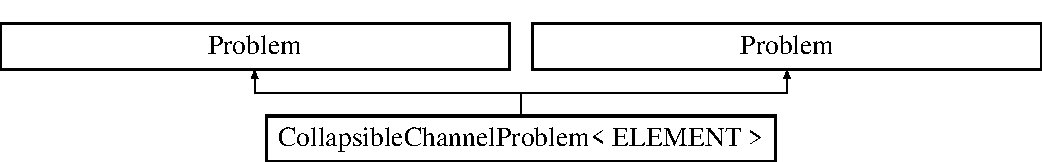
\includegraphics[height=2.000000cm]{classCollapsibleChannelProblem}
\end{center}
\end{figure}
\subsection*{Public Member Functions}
\begin{DoxyCompactItemize}
\item 
\hyperlink{classCollapsibleChannelProblem_ab43fa30667f57e8019c8b30fd93156f8}{Collapsible\+Channel\+Problem} (const unsigned \&nup, const unsigned \&ncollapsible, const unsigned \&ndown, const unsigned \&ny, const double \&lup, const double \&lcollapsible, const double \&ldown, const double \&ly, const double \&amplitude, const double \&period)
\begin{DoxyCompactList}\small\item\em Constructor \+: the arguments are the number of elements, the length of the domain and the amplitude and period of the oscillations. \end{DoxyCompactList}\item 
\hyperlink{classCollapsibleChannelProblem_a205e3e654d3205d1d55ac46e7b63ca9d}{$\sim$\+Collapsible\+Channel\+Problem} ()
\begin{DoxyCompactList}\small\item\em Empty destructor. \end{DoxyCompactList}\item 
Refineable\+Collapsible\+Channel\+Mesh$<$ E\+L\+E\+M\+E\+NT $>$ $\ast$ \hyperlink{classCollapsibleChannelProblem_a49a428b5f489d11b3fb92199b72f6dd7}{bulk\+\_\+mesh\+\_\+pt} ()
\begin{DoxyCompactList}\small\item\em Access function for the specific mesh. \end{DoxyCompactList}\item 
void \hyperlink{classCollapsibleChannelProblem_ad7597f95eb755184ec1f9581c713ff78}{actions\+\_\+before\+\_\+newton\+\_\+solve} ()
\begin{DoxyCompactList}\small\item\em Update the problem specs before solve (empty) \end{DoxyCompactList}\item 
void \hyperlink{classCollapsibleChannelProblem_a34299672cba0f3c1db3901427eb4da4a}{actions\+\_\+after\+\_\+newton\+\_\+solve} ()
\begin{DoxyCompactList}\small\item\em Update the problem after solve (empty) \end{DoxyCompactList}\item 
void \hyperlink{classCollapsibleChannelProblem_a4c365050b11c184007b8e1cd6079147f}{actions\+\_\+before\+\_\+implicit\+\_\+timestep} ()
\begin{DoxyCompactList}\small\item\em Update the velocity boundary condition on the moving wall. \end{DoxyCompactList}\item 
void \hyperlink{classCollapsibleChannelProblem_a54abc5259d590154e5dfa458d885c16c}{actions\+\_\+before\+\_\+adapt} ()
\begin{DoxyCompactList}\small\item\em Actions before adapt\+: Wipe the mesh of prescribed traction elements. \end{DoxyCompactList}\item 
void \hyperlink{classCollapsibleChannelProblem_a3ea01d83f0256c588a652741c6c33e0e}{actions\+\_\+after\+\_\+adapt} ()
\begin{DoxyCompactList}\small\item\em Actions after adapt\+: Rebuild the mesh of prescribed traction elements. \end{DoxyCompactList}\item 
void \hyperlink{classCollapsibleChannelProblem_a646147fb75669cfcc5bb56ee79d9b8da}{set\+\_\+initial\+\_\+condition} ()
\begin{DoxyCompactList}\small\item\em Apply initial conditions. \end{DoxyCompactList}\item 
void \hyperlink{classCollapsibleChannelProblem_afc4af9796c01d904d4074bd5bbfc5b9b}{doc\+\_\+solution} (Doc\+Info \&doc\+\_\+info, ofstream \&trace\+\_\+file)
\begin{DoxyCompactList}\small\item\em Doc the solution. \end{DoxyCompactList}\item 
\hyperlink{classCollapsibleChannelProblem_ab43fa30667f57e8019c8b30fd93156f8}{Collapsible\+Channel\+Problem} (const unsigned \&nup, const unsigned \&ncollapsible, const unsigned \&ndown, const unsigned \&ny, const double \&lup, const double \&lcollapsible, const double \&ldown, const double \&ly, const double \&amplitude, const double \&period)
\begin{DoxyCompactList}\small\item\em Constructor \+: the arguments are the number of elements, the length of the domain and the amplitude and period of the oscillations. \end{DoxyCompactList}\item 
\hyperlink{classCollapsibleChannelProblem_a205e3e654d3205d1d55ac46e7b63ca9d}{$\sim$\+Collapsible\+Channel\+Problem} ()
\begin{DoxyCompactList}\small\item\em Empty destructor. \end{DoxyCompactList}\item 
\hyperlink{classoomph_1_1MyRefineableAlgebraicCollapsibleChannelMesh}{My\+Refineable\+Algebraic\+Collapsible\+Channel\+Mesh}$<$ E\+L\+E\+M\+E\+NT $>$ $\ast$ \hyperlink{classCollapsibleChannelProblem_abe1a38b5c84188910435874511a877f6}{bulk\+\_\+mesh\+\_\+pt} ()
\begin{DoxyCompactList}\small\item\em Access function for the specific mesh. \end{DoxyCompactList}\item 
\hyperlink{classoomph_1_1MyAlgebraicCollapsibleChannelMesh}{My\+Algebraic\+Collapsible\+Channel\+Mesh}$<$ E\+L\+E\+M\+E\+NT $>$ $\ast$ \hyperlink{classCollapsibleChannelProblem_a411441ab7ac76c04613b1a7f558a6621}{bulk\+\_\+mesh\+\_\+pt} ()
\begin{DoxyCompactList}\small\item\em Access function for the specific mesh. \end{DoxyCompactList}\item 
void \hyperlink{classCollapsibleChannelProblem_ad7597f95eb755184ec1f9581c713ff78}{actions\+\_\+before\+\_\+newton\+\_\+solve} ()
\begin{DoxyCompactList}\small\item\em Update the problem specs before solve (empty) \end{DoxyCompactList}\item 
void \hyperlink{classCollapsibleChannelProblem_a34299672cba0f3c1db3901427eb4da4a}{actions\+\_\+after\+\_\+newton\+\_\+solve} ()
\begin{DoxyCompactList}\small\item\em Update the problem after solve (empty) \end{DoxyCompactList}\item 
void \hyperlink{classCollapsibleChannelProblem_a4c365050b11c184007b8e1cd6079147f}{actions\+\_\+before\+\_\+implicit\+\_\+timestep} ()
\begin{DoxyCompactList}\small\item\em Update the velocity boundary condition on the moving wall. \end{DoxyCompactList}\item 
void \hyperlink{classCollapsibleChannelProblem_a54abc5259d590154e5dfa458d885c16c}{actions\+\_\+before\+\_\+adapt} ()
\begin{DoxyCompactList}\small\item\em Actions before adapt\+: Wipe the mesh of prescribed traction elements. \end{DoxyCompactList}\item 
void \hyperlink{classCollapsibleChannelProblem_a3ea01d83f0256c588a652741c6c33e0e}{actions\+\_\+after\+\_\+adapt} ()
\begin{DoxyCompactList}\small\item\em Actions after adapt\+: Rebuild the mesh of prescribed traction elements. \end{DoxyCompactList}\item 
void \hyperlink{classCollapsibleChannelProblem_a646147fb75669cfcc5bb56ee79d9b8da}{set\+\_\+initial\+\_\+condition} ()
\begin{DoxyCompactList}\small\item\em Apply initial conditions. \end{DoxyCompactList}\item 
void \hyperlink{classCollapsibleChannelProblem_afc4af9796c01d904d4074bd5bbfc5b9b}{doc\+\_\+solution} (Doc\+Info \&doc\+\_\+info, ofstream \&trace\+\_\+file)
\begin{DoxyCompactList}\small\item\em Doc the solution. \end{DoxyCompactList}\end{DoxyCompactItemize}
\subsection*{Private Member Functions}
\begin{DoxyCompactItemize}
\item 
void \hyperlink{classCollapsibleChannelProblem_a70cfe97c12c0cb6a2a81266cdd4d6088}{create\+\_\+traction\+\_\+elements} (const unsigned \&b, Mesh $\ast$const \&\hyperlink{classCollapsibleChannelProblem_a49a428b5f489d11b3fb92199b72f6dd7}{bulk\+\_\+mesh\+\_\+pt}, Mesh $\ast$const \&surface\+\_\+mesh\+\_\+pt)
\begin{DoxyCompactList}\small\item\em Create the traction elements. \end{DoxyCompactList}\item 
void \hyperlink{classCollapsibleChannelProblem_a6a5324dd1efb8c517a7e4d431b10fca4}{delete\+\_\+traction\+\_\+elements} (Mesh $\ast$const \&surface\+\_\+mesh\+\_\+pt)
\begin{DoxyCompactList}\small\item\em Delete prescribed traction elements from the surface mesh. \end{DoxyCompactList}\item 
void \hyperlink{classCollapsibleChannelProblem_a70cfe97c12c0cb6a2a81266cdd4d6088}{create\+\_\+traction\+\_\+elements} (const unsigned \&b, Mesh $\ast$const \&\hyperlink{classCollapsibleChannelProblem_a49a428b5f489d11b3fb92199b72f6dd7}{bulk\+\_\+mesh\+\_\+pt}, Mesh $\ast$const \&surface\+\_\+mesh\+\_\+pt)
\item 
void \hyperlink{classCollapsibleChannelProblem_a6a5324dd1efb8c517a7e4d431b10fca4}{delete\+\_\+traction\+\_\+elements} (Mesh $\ast$const \&surface\+\_\+mesh\+\_\+pt)
\begin{DoxyCompactList}\small\item\em Delete prescribed traction elements from the surface mesh. \end{DoxyCompactList}\end{DoxyCompactItemize}
\subsection*{Private Attributes}
\begin{DoxyCompactItemize}
\item 
unsigned \hyperlink{classCollapsibleChannelProblem_a512e07ac795b19bfed9f82fd7927e8f9}{Nup}
\begin{DoxyCompactList}\small\item\em Number of elements in the x direction in the upstream part of the channel. \end{DoxyCompactList}\item 
unsigned \hyperlink{classCollapsibleChannelProblem_a941d6703a949d3a2f73b24080ca34bab}{Ncollapsible}
\begin{DoxyCompactList}\small\item\em Number of elements in the x direction in the \char`\"{}collapsible\char`\"{} part of the channel. \end{DoxyCompactList}\item 
unsigned \hyperlink{classCollapsibleChannelProblem_ac3991835635f02f895ea35adc7d985dc}{Ndown}
\begin{DoxyCompactList}\small\item\em Number of elements in the x direction in the downstream part of the channel. \end{DoxyCompactList}\item 
unsigned \hyperlink{classCollapsibleChannelProblem_aca26ffb5de27680b8eb2195f05c8ff7d}{Ny}
\begin{DoxyCompactList}\small\item\em Number of elements across the channel. \end{DoxyCompactList}\item 
double \hyperlink{classCollapsibleChannelProblem_a56353f52e7cf1564ffe77373ead3c2d0}{Lup}
\begin{DoxyCompactList}\small\item\em x-\/length in the upstream part of the channel \end{DoxyCompactList}\item 
double \hyperlink{classCollapsibleChannelProblem_a4edf74f18e84c3a2170428322d9e6824}{Lcollapsible}
\begin{DoxyCompactList}\small\item\em x-\/length in the \char`\"{}collapsible\char`\"{} part of the channel \end{DoxyCompactList}\item 
double \hyperlink{classCollapsibleChannelProblem_a5beb774a744bc7b7b1b821cb96bb445e}{Ldown}
\begin{DoxyCompactList}\small\item\em x-\/length in the downstream part of the channel \end{DoxyCompactList}\item 
double \hyperlink{classCollapsibleChannelProblem_a7d600ad0b7326eda8d3bcbfde97b40cd}{Ly}
\begin{DoxyCompactList}\small\item\em Transverse length. \end{DoxyCompactList}\item 
\hyperlink{classOscillatingWall}{Oscillating\+Wall} $\ast$ \hyperlink{classCollapsibleChannelProblem_a54065436b8f884469ed80eae6fe67a5c}{Wall\+\_\+pt}
\begin{DoxyCompactList}\small\item\em Pointer to the geometric object that parametrises the \char`\"{}collapsible\char`\"{} wall. \end{DoxyCompactList}\item 
Refineable\+Collapsible\+Channel\+Mesh$<$ E\+L\+E\+M\+E\+NT $>$ $\ast$ \hyperlink{classCollapsibleChannelProblem_acd96e5a1d72cc3a1aad196c97dcb3883}{Bulk\+\_\+mesh\+\_\+pt}
\begin{DoxyCompactList}\small\item\em Pointer to the \char`\"{}bulk\char`\"{} mesh. \end{DoxyCompactList}\item 
Mesh $\ast$ \hyperlink{classCollapsibleChannelProblem_a29f213b46b1c34851ff74e937444d04e}{Surface\+\_\+mesh\+\_\+pt}
\begin{DoxyCompactList}\small\item\em Pointer to the \char`\"{}surface\char`\"{} mesh that contains the applied traction elements. \end{DoxyCompactList}\item 
Node $\ast$ \hyperlink{classCollapsibleChannelProblem_a479d0dce7e090898f696505927a56cf8}{Left\+\_\+node\+\_\+pt}
\begin{DoxyCompactList}\small\item\em Pointer to the left control node. \end{DoxyCompactList}\item 
Node $\ast$ \hyperlink{classCollapsibleChannelProblem_ae02af6e90ea562b9fd8091bdd1ff972f}{Right\+\_\+node\+\_\+pt}
\begin{DoxyCompactList}\small\item\em Pointer to right control node. \end{DoxyCompactList}\item 
\hyperlink{classoomph_1_1MyAlgebraicCollapsibleChannelMesh}{My\+Algebraic\+Collapsible\+Channel\+Mesh}$<$ E\+L\+E\+M\+E\+NT $>$ $\ast$ \hyperlink{classCollapsibleChannelProblem_a0c3c4c226afe7d14f6967ac6d28ff15f}{Bulk\+\_\+mesh\+\_\+pt}
\begin{DoxyCompactList}\small\item\em Pointer to the \char`\"{}bulk\char`\"{} mesh. \end{DoxyCompactList}\end{DoxyCompactItemize}


\subsection{Detailed Description}
\subsubsection*{template$<$class E\+L\+E\+M\+E\+NT$>$\newline
class Collapsible\+Channel\+Problem$<$ E\+L\+E\+M\+E\+N\+T $>$}

Problem class. 

Definition at line 239 of file collapsible\+\_\+channel.\+cc.



\subsection{Constructor \& Destructor Documentation}
\mbox{\Hypertarget{classCollapsibleChannelProblem_ab43fa30667f57e8019c8b30fd93156f8}\label{classCollapsibleChannelProblem_ab43fa30667f57e8019c8b30fd93156f8}} 
\index{Collapsible\+Channel\+Problem@{Collapsible\+Channel\+Problem}!Collapsible\+Channel\+Problem@{Collapsible\+Channel\+Problem}}
\index{Collapsible\+Channel\+Problem@{Collapsible\+Channel\+Problem}!Collapsible\+Channel\+Problem@{Collapsible\+Channel\+Problem}}
\subsubsection{\texorpdfstring{Collapsible\+Channel\+Problem()}{CollapsibleChannelProblem()}\hspace{0.1cm}{\footnotesize\ttfamily [1/2]}}
{\footnotesize\ttfamily template$<$class E\+L\+E\+M\+E\+NT $>$ \\
\hyperlink{classCollapsibleChannelProblem}{Collapsible\+Channel\+Problem}$<$ E\+L\+E\+M\+E\+NT $>$\+::\hyperlink{classCollapsibleChannelProblem}{Collapsible\+Channel\+Problem} (\begin{DoxyParamCaption}\item[{const unsigned \&}]{nup,  }\item[{const unsigned \&}]{ncollapsible,  }\item[{const unsigned \&}]{ndown,  }\item[{const unsigned \&}]{ny,  }\item[{const double \&}]{lup,  }\item[{const double \&}]{lcollapsible,  }\item[{const double \&}]{ldown,  }\item[{const double \&}]{ly,  }\item[{const double \&}]{amplitude,  }\item[{const double \&}]{period }\end{DoxyParamCaption})}



Constructor \+: the arguments are the number of elements, the length of the domain and the amplitude and period of the oscillations. 

Constructor for the collapsible channel problem. 

Definition at line 354 of file collapsible\+\_\+channel.\+cc.



References Global\+\_\+\+Physical\+\_\+\+Variables\+::prescribed\+\_\+traction(), Global\+\_\+\+Physical\+\_\+\+Variables\+::\+Re, Global\+\_\+\+Physical\+\_\+\+Variables\+::\+Re\+St, and B\+L\+\_\+\+Squash\+::squash\+\_\+fct().

\mbox{\Hypertarget{classCollapsibleChannelProblem_a205e3e654d3205d1d55ac46e7b63ca9d}\label{classCollapsibleChannelProblem_a205e3e654d3205d1d55ac46e7b63ca9d}} 
\index{Collapsible\+Channel\+Problem@{Collapsible\+Channel\+Problem}!````~Collapsible\+Channel\+Problem@{$\sim$\+Collapsible\+Channel\+Problem}}
\index{````~Collapsible\+Channel\+Problem@{$\sim$\+Collapsible\+Channel\+Problem}!Collapsible\+Channel\+Problem@{Collapsible\+Channel\+Problem}}
\subsubsection{\texorpdfstring{$\sim$\+Collapsible\+Channel\+Problem()}{~CollapsibleChannelProblem()}\hspace{0.1cm}{\footnotesize\ttfamily [1/2]}}
{\footnotesize\ttfamily template$<$class E\+L\+E\+M\+E\+NT$>$ \\
\hyperlink{classCollapsibleChannelProblem}{Collapsible\+Channel\+Problem}$<$ E\+L\+E\+M\+E\+NT $>$\+::$\sim$\hyperlink{classCollapsibleChannelProblem}{Collapsible\+Channel\+Problem} (\begin{DoxyParamCaption}{ }\end{DoxyParamCaption})\hspace{0.3cm}{\ttfamily [inline]}}



Empty destructor. 



Definition at line 259 of file collapsible\+\_\+channel.\+cc.

\mbox{\Hypertarget{classCollapsibleChannelProblem_ab43fa30667f57e8019c8b30fd93156f8}\label{classCollapsibleChannelProblem_ab43fa30667f57e8019c8b30fd93156f8}} 
\index{Collapsible\+Channel\+Problem@{Collapsible\+Channel\+Problem}!Collapsible\+Channel\+Problem@{Collapsible\+Channel\+Problem}}
\index{Collapsible\+Channel\+Problem@{Collapsible\+Channel\+Problem}!Collapsible\+Channel\+Problem@{Collapsible\+Channel\+Problem}}
\subsubsection{\texorpdfstring{Collapsible\+Channel\+Problem()}{CollapsibleChannelProblem()}\hspace{0.1cm}{\footnotesize\ttfamily [2/2]}}
{\footnotesize\ttfamily template$<$class E\+L\+E\+M\+E\+NT$>$ \\
\hyperlink{classCollapsibleChannelProblem}{Collapsible\+Channel\+Problem}$<$ E\+L\+E\+M\+E\+NT $>$\+::\hyperlink{classCollapsibleChannelProblem}{Collapsible\+Channel\+Problem} (\begin{DoxyParamCaption}\item[{const unsigned \&}]{nup,  }\item[{const unsigned \&}]{ncollapsible,  }\item[{const unsigned \&}]{ndown,  }\item[{const unsigned \&}]{ny,  }\item[{const double \&}]{lup,  }\item[{const double \&}]{lcollapsible,  }\item[{const double \&}]{ldown,  }\item[{const double \&}]{ly,  }\item[{const double \&}]{amplitude,  }\item[{const double \&}]{period }\end{DoxyParamCaption})}



Constructor \+: the arguments are the number of elements, the length of the domain and the amplitude and period of the oscillations. 

\mbox{\Hypertarget{classCollapsibleChannelProblem_a205e3e654d3205d1d55ac46e7b63ca9d}\label{classCollapsibleChannelProblem_a205e3e654d3205d1d55ac46e7b63ca9d}} 
\index{Collapsible\+Channel\+Problem@{Collapsible\+Channel\+Problem}!````~Collapsible\+Channel\+Problem@{$\sim$\+Collapsible\+Channel\+Problem}}
\index{````~Collapsible\+Channel\+Problem@{$\sim$\+Collapsible\+Channel\+Problem}!Collapsible\+Channel\+Problem@{Collapsible\+Channel\+Problem}}
\subsubsection{\texorpdfstring{$\sim$\+Collapsible\+Channel\+Problem()}{~CollapsibleChannelProblem()}\hspace{0.1cm}{\footnotesize\ttfamily [2/2]}}
{\footnotesize\ttfamily template$<$class E\+L\+E\+M\+E\+NT$>$ \\
\hyperlink{classCollapsibleChannelProblem}{Collapsible\+Channel\+Problem}$<$ E\+L\+E\+M\+E\+NT $>$\+::$\sim$\hyperlink{classCollapsibleChannelProblem}{Collapsible\+Channel\+Problem} (\begin{DoxyParamCaption}{ }\end{DoxyParamCaption})\hspace{0.3cm}{\ttfamily [inline]}}



Empty destructor. 



Definition at line 260 of file collapsible\+\_\+channel\+\_\+algebraic.\+cc.



\subsection{Member Function Documentation}
\mbox{\Hypertarget{classCollapsibleChannelProblem_a3ea01d83f0256c588a652741c6c33e0e}\label{classCollapsibleChannelProblem_a3ea01d83f0256c588a652741c6c33e0e}} 
\index{Collapsible\+Channel\+Problem@{Collapsible\+Channel\+Problem}!actions\+\_\+after\+\_\+adapt@{actions\+\_\+after\+\_\+adapt}}
\index{actions\+\_\+after\+\_\+adapt@{actions\+\_\+after\+\_\+adapt}!Collapsible\+Channel\+Problem@{Collapsible\+Channel\+Problem}}
\subsubsection{\texorpdfstring{actions\+\_\+after\+\_\+adapt()}{actions\_after\_adapt()}\hspace{0.1cm}{\footnotesize\ttfamily [1/2]}}
{\footnotesize\ttfamily template$<$class E\+L\+E\+M\+E\+NT $>$ \\
void \hyperlink{classCollapsibleChannelProblem}{Collapsible\+Channel\+Problem}$<$ E\+L\+E\+M\+E\+NT $>$\+::actions\+\_\+after\+\_\+adapt (\begin{DoxyParamCaption}{ }\end{DoxyParamCaption})}



Actions after adapt\+: Rebuild the mesh of prescribed traction elements. 



Definition at line 745 of file collapsible\+\_\+channel.\+cc.



References Global\+\_\+\+Physical\+\_\+\+Variables\+::prescribed\+\_\+traction().

\mbox{\Hypertarget{classCollapsibleChannelProblem_a3ea01d83f0256c588a652741c6c33e0e}\label{classCollapsibleChannelProblem_a3ea01d83f0256c588a652741c6c33e0e}} 
\index{Collapsible\+Channel\+Problem@{Collapsible\+Channel\+Problem}!actions\+\_\+after\+\_\+adapt@{actions\+\_\+after\+\_\+adapt}}
\index{actions\+\_\+after\+\_\+adapt@{actions\+\_\+after\+\_\+adapt}!Collapsible\+Channel\+Problem@{Collapsible\+Channel\+Problem}}
\subsubsection{\texorpdfstring{actions\+\_\+after\+\_\+adapt()}{actions\_after\_adapt()}\hspace{0.1cm}{\footnotesize\ttfamily [2/2]}}
{\footnotesize\ttfamily template$<$class E\+L\+E\+M\+E\+NT$>$ \\
void \hyperlink{classCollapsibleChannelProblem}{Collapsible\+Channel\+Problem}$<$ E\+L\+E\+M\+E\+NT $>$\+::actions\+\_\+after\+\_\+adapt (\begin{DoxyParamCaption}{ }\end{DoxyParamCaption})}



Actions after adapt\+: Rebuild the mesh of prescribed traction elements. 

\mbox{\Hypertarget{classCollapsibleChannelProblem_a34299672cba0f3c1db3901427eb4da4a}\label{classCollapsibleChannelProblem_a34299672cba0f3c1db3901427eb4da4a}} 
\index{Collapsible\+Channel\+Problem@{Collapsible\+Channel\+Problem}!actions\+\_\+after\+\_\+newton\+\_\+solve@{actions\+\_\+after\+\_\+newton\+\_\+solve}}
\index{actions\+\_\+after\+\_\+newton\+\_\+solve@{actions\+\_\+after\+\_\+newton\+\_\+solve}!Collapsible\+Channel\+Problem@{Collapsible\+Channel\+Problem}}
\subsubsection{\texorpdfstring{actions\+\_\+after\+\_\+newton\+\_\+solve()}{actions\_after\_newton\_solve()}\hspace{0.1cm}{\footnotesize\ttfamily [1/2]}}
{\footnotesize\ttfamily template$<$class E\+L\+E\+M\+E\+NT$>$ \\
void \hyperlink{classCollapsibleChannelProblem}{Collapsible\+Channel\+Problem}$<$ E\+L\+E\+M\+E\+NT $>$\+::actions\+\_\+after\+\_\+newton\+\_\+solve (\begin{DoxyParamCaption}{ }\end{DoxyParamCaption})\hspace{0.3cm}{\ttfamily [inline]}}



Update the problem after solve (empty) 



Definition at line 276 of file collapsible\+\_\+channel.\+cc.

\mbox{\Hypertarget{classCollapsibleChannelProblem_a34299672cba0f3c1db3901427eb4da4a}\label{classCollapsibleChannelProblem_a34299672cba0f3c1db3901427eb4da4a}} 
\index{Collapsible\+Channel\+Problem@{Collapsible\+Channel\+Problem}!actions\+\_\+after\+\_\+newton\+\_\+solve@{actions\+\_\+after\+\_\+newton\+\_\+solve}}
\index{actions\+\_\+after\+\_\+newton\+\_\+solve@{actions\+\_\+after\+\_\+newton\+\_\+solve}!Collapsible\+Channel\+Problem@{Collapsible\+Channel\+Problem}}
\subsubsection{\texorpdfstring{actions\+\_\+after\+\_\+newton\+\_\+solve()}{actions\_after\_newton\_solve()}\hspace{0.1cm}{\footnotesize\ttfamily [2/2]}}
{\footnotesize\ttfamily template$<$class E\+L\+E\+M\+E\+NT$>$ \\
void \hyperlink{classCollapsibleChannelProblem}{Collapsible\+Channel\+Problem}$<$ E\+L\+E\+M\+E\+NT $>$\+::actions\+\_\+after\+\_\+newton\+\_\+solve (\begin{DoxyParamCaption}{ }\end{DoxyParamCaption})\hspace{0.3cm}{\ttfamily [inline]}}



Update the problem after solve (empty) 



Definition at line 296 of file collapsible\+\_\+channel\+\_\+algebraic.\+cc.

\mbox{\Hypertarget{classCollapsibleChannelProblem_a54abc5259d590154e5dfa458d885c16c}\label{classCollapsibleChannelProblem_a54abc5259d590154e5dfa458d885c16c}} 
\index{Collapsible\+Channel\+Problem@{Collapsible\+Channel\+Problem}!actions\+\_\+before\+\_\+adapt@{actions\+\_\+before\+\_\+adapt}}
\index{actions\+\_\+before\+\_\+adapt@{actions\+\_\+before\+\_\+adapt}!Collapsible\+Channel\+Problem@{Collapsible\+Channel\+Problem}}
\subsubsection{\texorpdfstring{actions\+\_\+before\+\_\+adapt()}{actions\_before\_adapt()}\hspace{0.1cm}{\footnotesize\ttfamily [1/2]}}
{\footnotesize\ttfamily template$<$class E\+L\+E\+M\+E\+NT $>$ \\
void \hyperlink{classCollapsibleChannelProblem}{Collapsible\+Channel\+Problem}$<$ E\+L\+E\+M\+E\+NT $>$\+::actions\+\_\+before\+\_\+adapt (\begin{DoxyParamCaption}{ }\end{DoxyParamCaption})}



Actions before adapt\+: Wipe the mesh of prescribed traction elements. 



Definition at line 730 of file collapsible\+\_\+channel.\+cc.

\mbox{\Hypertarget{classCollapsibleChannelProblem_a54abc5259d590154e5dfa458d885c16c}\label{classCollapsibleChannelProblem_a54abc5259d590154e5dfa458d885c16c}} 
\index{Collapsible\+Channel\+Problem@{Collapsible\+Channel\+Problem}!actions\+\_\+before\+\_\+adapt@{actions\+\_\+before\+\_\+adapt}}
\index{actions\+\_\+before\+\_\+adapt@{actions\+\_\+before\+\_\+adapt}!Collapsible\+Channel\+Problem@{Collapsible\+Channel\+Problem}}
\subsubsection{\texorpdfstring{actions\+\_\+before\+\_\+adapt()}{actions\_before\_adapt()}\hspace{0.1cm}{\footnotesize\ttfamily [2/2]}}
{\footnotesize\ttfamily template$<$class E\+L\+E\+M\+E\+NT$>$ \\
void \hyperlink{classCollapsibleChannelProblem}{Collapsible\+Channel\+Problem}$<$ E\+L\+E\+M\+E\+NT $>$\+::actions\+\_\+before\+\_\+adapt (\begin{DoxyParamCaption}{ }\end{DoxyParamCaption})}



Actions before adapt\+: Wipe the mesh of prescribed traction elements. 

\mbox{\Hypertarget{classCollapsibleChannelProblem_a4c365050b11c184007b8e1cd6079147f}\label{classCollapsibleChannelProblem_a4c365050b11c184007b8e1cd6079147f}} 
\index{Collapsible\+Channel\+Problem@{Collapsible\+Channel\+Problem}!actions\+\_\+before\+\_\+implicit\+\_\+timestep@{actions\+\_\+before\+\_\+implicit\+\_\+timestep}}
\index{actions\+\_\+before\+\_\+implicit\+\_\+timestep@{actions\+\_\+before\+\_\+implicit\+\_\+timestep}!Collapsible\+Channel\+Problem@{Collapsible\+Channel\+Problem}}
\subsubsection{\texorpdfstring{actions\+\_\+before\+\_\+implicit\+\_\+timestep()}{actions\_before\_implicit\_timestep()}\hspace{0.1cm}{\footnotesize\ttfamily [1/2]}}
{\footnotesize\ttfamily template$<$class E\+L\+E\+M\+E\+NT $>$ \\
void \hyperlink{classCollapsibleChannelProblem}{Collapsible\+Channel\+Problem}$<$ E\+L\+E\+M\+E\+NT $>$\+::actions\+\_\+before\+\_\+implicit\+\_\+timestep (\begin{DoxyParamCaption}{ }\end{DoxyParamCaption})}



Update the velocity boundary condition on the moving wall. 

Execute the actions before timestep\+: Update the velocity boundary condition on the moving wall 

Definition at line 704 of file collapsible\+\_\+channel.\+cc.

\mbox{\Hypertarget{classCollapsibleChannelProblem_a4c365050b11c184007b8e1cd6079147f}\label{classCollapsibleChannelProblem_a4c365050b11c184007b8e1cd6079147f}} 
\index{Collapsible\+Channel\+Problem@{Collapsible\+Channel\+Problem}!actions\+\_\+before\+\_\+implicit\+\_\+timestep@{actions\+\_\+before\+\_\+implicit\+\_\+timestep}}
\index{actions\+\_\+before\+\_\+implicit\+\_\+timestep@{actions\+\_\+before\+\_\+implicit\+\_\+timestep}!Collapsible\+Channel\+Problem@{Collapsible\+Channel\+Problem}}
\subsubsection{\texorpdfstring{actions\+\_\+before\+\_\+implicit\+\_\+timestep()}{actions\_before\_implicit\_timestep()}\hspace{0.1cm}{\footnotesize\ttfamily [2/2]}}
{\footnotesize\ttfamily template$<$class E\+L\+E\+M\+E\+NT$>$ \\
void \hyperlink{classCollapsibleChannelProblem}{Collapsible\+Channel\+Problem}$<$ E\+L\+E\+M\+E\+NT $>$\+::actions\+\_\+before\+\_\+implicit\+\_\+timestep (\begin{DoxyParamCaption}{ }\end{DoxyParamCaption})}



Update the velocity boundary condition on the moving wall. 

\mbox{\Hypertarget{classCollapsibleChannelProblem_ad7597f95eb755184ec1f9581c713ff78}\label{classCollapsibleChannelProblem_ad7597f95eb755184ec1f9581c713ff78}} 
\index{Collapsible\+Channel\+Problem@{Collapsible\+Channel\+Problem}!actions\+\_\+before\+\_\+newton\+\_\+solve@{actions\+\_\+before\+\_\+newton\+\_\+solve}}
\index{actions\+\_\+before\+\_\+newton\+\_\+solve@{actions\+\_\+before\+\_\+newton\+\_\+solve}!Collapsible\+Channel\+Problem@{Collapsible\+Channel\+Problem}}
\subsubsection{\texorpdfstring{actions\+\_\+before\+\_\+newton\+\_\+solve()}{actions\_before\_newton\_solve()}\hspace{0.1cm}{\footnotesize\ttfamily [1/2]}}
{\footnotesize\ttfamily template$<$class E\+L\+E\+M\+E\+NT$>$ \\
void \hyperlink{classCollapsibleChannelProblem}{Collapsible\+Channel\+Problem}$<$ E\+L\+E\+M\+E\+NT $>$\+::actions\+\_\+before\+\_\+newton\+\_\+solve (\begin{DoxyParamCaption}{ }\end{DoxyParamCaption})\hspace{0.3cm}{\ttfamily [inline]}}



Update the problem specs before solve (empty) 



Definition at line 273 of file collapsible\+\_\+channel.\+cc.

\mbox{\Hypertarget{classCollapsibleChannelProblem_ad7597f95eb755184ec1f9581c713ff78}\label{classCollapsibleChannelProblem_ad7597f95eb755184ec1f9581c713ff78}} 
\index{Collapsible\+Channel\+Problem@{Collapsible\+Channel\+Problem}!actions\+\_\+before\+\_\+newton\+\_\+solve@{actions\+\_\+before\+\_\+newton\+\_\+solve}}
\index{actions\+\_\+before\+\_\+newton\+\_\+solve@{actions\+\_\+before\+\_\+newton\+\_\+solve}!Collapsible\+Channel\+Problem@{Collapsible\+Channel\+Problem}}
\subsubsection{\texorpdfstring{actions\+\_\+before\+\_\+newton\+\_\+solve()}{actions\_before\_newton\_solve()}\hspace{0.1cm}{\footnotesize\ttfamily [2/2]}}
{\footnotesize\ttfamily template$<$class E\+L\+E\+M\+E\+NT$>$ \\
void \hyperlink{classCollapsibleChannelProblem}{Collapsible\+Channel\+Problem}$<$ E\+L\+E\+M\+E\+NT $>$\+::actions\+\_\+before\+\_\+newton\+\_\+solve (\begin{DoxyParamCaption}{ }\end{DoxyParamCaption})\hspace{0.3cm}{\ttfamily [inline]}}



Update the problem specs before solve (empty) 



Definition at line 293 of file collapsible\+\_\+channel\+\_\+algebraic.\+cc.

\mbox{\Hypertarget{classCollapsibleChannelProblem_a49a428b5f489d11b3fb92199b72f6dd7}\label{classCollapsibleChannelProblem_a49a428b5f489d11b3fb92199b72f6dd7}} 
\index{Collapsible\+Channel\+Problem@{Collapsible\+Channel\+Problem}!bulk\+\_\+mesh\+\_\+pt@{bulk\+\_\+mesh\+\_\+pt}}
\index{bulk\+\_\+mesh\+\_\+pt@{bulk\+\_\+mesh\+\_\+pt}!Collapsible\+Channel\+Problem@{Collapsible\+Channel\+Problem}}
\subsubsection{\texorpdfstring{bulk\+\_\+mesh\+\_\+pt()}{bulk\_mesh\_pt()}\hspace{0.1cm}{\footnotesize\ttfamily [1/3]}}
{\footnotesize\ttfamily template$<$class E\+L\+E\+M\+E\+NT$>$ \\
Refineable\+Collapsible\+Channel\+Mesh$<$E\+L\+E\+M\+E\+NT$>$$\ast$ \hyperlink{classCollapsibleChannelProblem}{Collapsible\+Channel\+Problem}$<$ E\+L\+E\+M\+E\+NT $>$\+::bulk\+\_\+mesh\+\_\+pt (\begin{DoxyParamCaption}{ }\end{DoxyParamCaption})\hspace{0.3cm}{\ttfamily [inline]}}



Access function for the specific mesh. 



Definition at line 262 of file collapsible\+\_\+channel.\+cc.



Referenced by main().

\mbox{\Hypertarget{classCollapsibleChannelProblem_abe1a38b5c84188910435874511a877f6}\label{classCollapsibleChannelProblem_abe1a38b5c84188910435874511a877f6}} 
\index{Collapsible\+Channel\+Problem@{Collapsible\+Channel\+Problem}!bulk\+\_\+mesh\+\_\+pt@{bulk\+\_\+mesh\+\_\+pt}}
\index{bulk\+\_\+mesh\+\_\+pt@{bulk\+\_\+mesh\+\_\+pt}!Collapsible\+Channel\+Problem@{Collapsible\+Channel\+Problem}}
\subsubsection{\texorpdfstring{bulk\+\_\+mesh\+\_\+pt()}{bulk\_mesh\_pt()}\hspace{0.1cm}{\footnotesize\ttfamily [2/3]}}
{\footnotesize\ttfamily template$<$class E\+L\+E\+M\+E\+NT$>$ \\
\hyperlink{classoomph_1_1MyRefineableAlgebraicCollapsibleChannelMesh}{My\+Refineable\+Algebraic\+Collapsible\+Channel\+Mesh}$<$E\+L\+E\+M\+E\+NT$>$$\ast$ \hyperlink{classCollapsibleChannelProblem}{Collapsible\+Channel\+Problem}$<$ E\+L\+E\+M\+E\+NT $>$\+::bulk\+\_\+mesh\+\_\+pt (\begin{DoxyParamCaption}{ }\end{DoxyParamCaption})\hspace{0.3cm}{\ttfamily [inline]}}



Access function for the specific mesh. 



Definition at line 266 of file collapsible\+\_\+channel\+\_\+algebraic.\+cc.

\mbox{\Hypertarget{classCollapsibleChannelProblem_a411441ab7ac76c04613b1a7f558a6621}\label{classCollapsibleChannelProblem_a411441ab7ac76c04613b1a7f558a6621}} 
\index{Collapsible\+Channel\+Problem@{Collapsible\+Channel\+Problem}!bulk\+\_\+mesh\+\_\+pt@{bulk\+\_\+mesh\+\_\+pt}}
\index{bulk\+\_\+mesh\+\_\+pt@{bulk\+\_\+mesh\+\_\+pt}!Collapsible\+Channel\+Problem@{Collapsible\+Channel\+Problem}}
\subsubsection{\texorpdfstring{bulk\+\_\+mesh\+\_\+pt()}{bulk\_mesh\_pt()}\hspace{0.1cm}{\footnotesize\ttfamily [3/3]}}
{\footnotesize\ttfamily template$<$class E\+L\+E\+M\+E\+NT$>$ \\
\hyperlink{classoomph_1_1MyAlgebraicCollapsibleChannelMesh}{My\+Algebraic\+Collapsible\+Channel\+Mesh}$<$E\+L\+E\+M\+E\+NT$>$$\ast$ \hyperlink{classCollapsibleChannelProblem}{Collapsible\+Channel\+Problem}$<$ E\+L\+E\+M\+E\+NT $>$\+::bulk\+\_\+mesh\+\_\+pt (\begin{DoxyParamCaption}{ }\end{DoxyParamCaption})\hspace{0.3cm}{\ttfamily [inline]}}



Access function for the specific mesh. 



Definition at line 279 of file collapsible\+\_\+channel\+\_\+algebraic.\+cc.

\mbox{\Hypertarget{classCollapsibleChannelProblem_a70cfe97c12c0cb6a2a81266cdd4d6088}\label{classCollapsibleChannelProblem_a70cfe97c12c0cb6a2a81266cdd4d6088}} 
\index{Collapsible\+Channel\+Problem@{Collapsible\+Channel\+Problem}!create\+\_\+traction\+\_\+elements@{create\+\_\+traction\+\_\+elements}}
\index{create\+\_\+traction\+\_\+elements@{create\+\_\+traction\+\_\+elements}!Collapsible\+Channel\+Problem@{Collapsible\+Channel\+Problem}}
\subsubsection{\texorpdfstring{create\+\_\+traction\+\_\+elements()}{create\_traction\_elements()}\hspace{0.1cm}{\footnotesize\ttfamily [1/2]}}
{\footnotesize\ttfamily template$<$class E\+L\+E\+M\+E\+NT $>$ \\
void \hyperlink{classCollapsibleChannelProblem}{Collapsible\+Channel\+Problem}$<$ E\+L\+E\+M\+E\+NT $>$\+::create\+\_\+traction\+\_\+elements (\begin{DoxyParamCaption}\item[{const unsigned \&}]{b,  }\item[{Mesh $\ast$const \&}]{bulk\+\_\+mesh\+\_\+pt,  }\item[{Mesh $\ast$const \&}]{surface\+\_\+mesh\+\_\+pt }\end{DoxyParamCaption})\hspace{0.3cm}{\ttfamily [private]}}



Create the traction elements. 

Create the prescribed traction elements on boundary b of the bulk mesh and stick them into the surface mesh. 

Definition at line 601 of file collapsible\+\_\+channel.\+cc.



References Collapsible\+Channel\+Problem$<$ E\+L\+E\+M\+E\+N\+T $>$\+::delete\+\_\+traction\+\_\+elements().

\mbox{\Hypertarget{classCollapsibleChannelProblem_a70cfe97c12c0cb6a2a81266cdd4d6088}\label{classCollapsibleChannelProblem_a70cfe97c12c0cb6a2a81266cdd4d6088}} 
\index{Collapsible\+Channel\+Problem@{Collapsible\+Channel\+Problem}!create\+\_\+traction\+\_\+elements@{create\+\_\+traction\+\_\+elements}}
\index{create\+\_\+traction\+\_\+elements@{create\+\_\+traction\+\_\+elements}!Collapsible\+Channel\+Problem@{Collapsible\+Channel\+Problem}}
\subsubsection{\texorpdfstring{create\+\_\+traction\+\_\+elements()}{create\_traction\_elements()}\hspace{0.1cm}{\footnotesize\ttfamily [2/2]}}
{\footnotesize\ttfamily template$<$class E\+L\+E\+M\+E\+NT$>$ \\
void \hyperlink{classCollapsibleChannelProblem}{Collapsible\+Channel\+Problem}$<$ E\+L\+E\+M\+E\+NT $>$\+::create\+\_\+traction\+\_\+elements (\begin{DoxyParamCaption}\item[{const unsigned \&}]{b,  }\item[{Mesh $\ast$const \&}]{bulk\+\_\+mesh\+\_\+pt,  }\item[{Mesh $\ast$const \&}]{surface\+\_\+mesh\+\_\+pt }\end{DoxyParamCaption})\hspace{0.3cm}{\ttfamily [private]}}

Create the prescribed traction elements on boundary b of the bulk mesh and stick them into the surface mesh. \mbox{\Hypertarget{classCollapsibleChannelProblem_a6a5324dd1efb8c517a7e4d431b10fca4}\label{classCollapsibleChannelProblem_a6a5324dd1efb8c517a7e4d431b10fca4}} 
\index{Collapsible\+Channel\+Problem@{Collapsible\+Channel\+Problem}!delete\+\_\+traction\+\_\+elements@{delete\+\_\+traction\+\_\+elements}}
\index{delete\+\_\+traction\+\_\+elements@{delete\+\_\+traction\+\_\+elements}!Collapsible\+Channel\+Problem@{Collapsible\+Channel\+Problem}}
\subsubsection{\texorpdfstring{delete\+\_\+traction\+\_\+elements()}{delete\_traction\_elements()}\hspace{0.1cm}{\footnotesize\ttfamily [1/2]}}
{\footnotesize\ttfamily template$<$class E\+L\+E\+M\+E\+NT $>$ \\
void \hyperlink{classCollapsibleChannelProblem}{Collapsible\+Channel\+Problem}$<$ E\+L\+E\+M\+E\+NT $>$\+::delete\+\_\+traction\+\_\+elements (\begin{DoxyParamCaption}\item[{Mesh $\ast$const \&}]{surface\+\_\+mesh\+\_\+pt }\end{DoxyParamCaption})\hspace{0.3cm}{\ttfamily [private]}}



Delete prescribed traction elements from the surface mesh. 

Delete traction elements and wipe the surface mesh. 

Definition at line 634 of file collapsible\+\_\+channel.\+cc.



Referenced by Collapsible\+Channel\+Problem$<$ E\+L\+E\+M\+E\+N\+T $>$\+::create\+\_\+traction\+\_\+elements().

\mbox{\Hypertarget{classCollapsibleChannelProblem_a6a5324dd1efb8c517a7e4d431b10fca4}\label{classCollapsibleChannelProblem_a6a5324dd1efb8c517a7e4d431b10fca4}} 
\index{Collapsible\+Channel\+Problem@{Collapsible\+Channel\+Problem}!delete\+\_\+traction\+\_\+elements@{delete\+\_\+traction\+\_\+elements}}
\index{delete\+\_\+traction\+\_\+elements@{delete\+\_\+traction\+\_\+elements}!Collapsible\+Channel\+Problem@{Collapsible\+Channel\+Problem}}
\subsubsection{\texorpdfstring{delete\+\_\+traction\+\_\+elements()}{delete\_traction\_elements()}\hspace{0.1cm}{\footnotesize\ttfamily [2/2]}}
{\footnotesize\ttfamily template$<$class E\+L\+E\+M\+E\+NT$>$ \\
void \hyperlink{classCollapsibleChannelProblem}{Collapsible\+Channel\+Problem}$<$ E\+L\+E\+M\+E\+NT $>$\+::delete\+\_\+traction\+\_\+elements (\begin{DoxyParamCaption}\item[{Mesh $\ast$const \&}]{surface\+\_\+mesh\+\_\+pt }\end{DoxyParamCaption})\hspace{0.3cm}{\ttfamily [private]}}



Delete prescribed traction elements from the surface mesh. 

\mbox{\Hypertarget{classCollapsibleChannelProblem_afc4af9796c01d904d4074bd5bbfc5b9b}\label{classCollapsibleChannelProblem_afc4af9796c01d904d4074bd5bbfc5b9b}} 
\index{Collapsible\+Channel\+Problem@{Collapsible\+Channel\+Problem}!doc\+\_\+solution@{doc\+\_\+solution}}
\index{doc\+\_\+solution@{doc\+\_\+solution}!Collapsible\+Channel\+Problem@{Collapsible\+Channel\+Problem}}
\subsubsection{\texorpdfstring{doc\+\_\+solution()}{doc\_solution()}\hspace{0.1cm}{\footnotesize\ttfamily [1/2]}}
{\footnotesize\ttfamily template$<$class E\+L\+E\+M\+E\+NT $>$ \\
void \hyperlink{classCollapsibleChannelProblem}{Collapsible\+Channel\+Problem}$<$ E\+L\+E\+M\+E\+NT $>$\+::doc\+\_\+solution (\begin{DoxyParamCaption}\item[{Doc\+Info \&}]{doc\+\_\+info,  }\item[{ofstream \&}]{trace\+\_\+file }\end{DoxyParamCaption})}



Doc the solution. 



Definition at line 547 of file collapsible\+\_\+channel.\+cc.



Referenced by main().

\mbox{\Hypertarget{classCollapsibleChannelProblem_afc4af9796c01d904d4074bd5bbfc5b9b}\label{classCollapsibleChannelProblem_afc4af9796c01d904d4074bd5bbfc5b9b}} 
\index{Collapsible\+Channel\+Problem@{Collapsible\+Channel\+Problem}!doc\+\_\+solution@{doc\+\_\+solution}}
\index{doc\+\_\+solution@{doc\+\_\+solution}!Collapsible\+Channel\+Problem@{Collapsible\+Channel\+Problem}}
\subsubsection{\texorpdfstring{doc\+\_\+solution()}{doc\_solution()}\hspace{0.1cm}{\footnotesize\ttfamily [2/2]}}
{\footnotesize\ttfamily template$<$class E\+L\+E\+M\+E\+NT$>$ \\
void \hyperlink{classCollapsibleChannelProblem}{Collapsible\+Channel\+Problem}$<$ E\+L\+E\+M\+E\+NT $>$\+::doc\+\_\+solution (\begin{DoxyParamCaption}\item[{Doc\+Info \&}]{doc\+\_\+info,  }\item[{ofstream \&}]{trace\+\_\+file }\end{DoxyParamCaption})}



Doc the solution. 

\mbox{\Hypertarget{classCollapsibleChannelProblem_a646147fb75669cfcc5bb56ee79d9b8da}\label{classCollapsibleChannelProblem_a646147fb75669cfcc5bb56ee79d9b8da}} 
\index{Collapsible\+Channel\+Problem@{Collapsible\+Channel\+Problem}!set\+\_\+initial\+\_\+condition@{set\+\_\+initial\+\_\+condition}}
\index{set\+\_\+initial\+\_\+condition@{set\+\_\+initial\+\_\+condition}!Collapsible\+Channel\+Problem@{Collapsible\+Channel\+Problem}}
\subsubsection{\texorpdfstring{set\+\_\+initial\+\_\+condition()}{set\_initial\_condition()}\hspace{0.1cm}{\footnotesize\ttfamily [1/2]}}
{\footnotesize\ttfamily template$<$class E\+L\+E\+M\+E\+NT $>$ \\
void \hyperlink{classCollapsibleChannelProblem}{Collapsible\+Channel\+Problem}$<$ E\+L\+E\+M\+E\+NT $>$\+::set\+\_\+initial\+\_\+condition (\begin{DoxyParamCaption}{ }\end{DoxyParamCaption})}



Apply initial conditions. 

Apply initial conditions\+: Impulsive start from steady Poiseuille.

Apply initial conditions\+: Impulsive start from steady Poiseuille flow. 

Definition at line 657 of file collapsible\+\_\+channel.\+cc.



Referenced by main().

\mbox{\Hypertarget{classCollapsibleChannelProblem_a646147fb75669cfcc5bb56ee79d9b8da}\label{classCollapsibleChannelProblem_a646147fb75669cfcc5bb56ee79d9b8da}} 
\index{Collapsible\+Channel\+Problem@{Collapsible\+Channel\+Problem}!set\+\_\+initial\+\_\+condition@{set\+\_\+initial\+\_\+condition}}
\index{set\+\_\+initial\+\_\+condition@{set\+\_\+initial\+\_\+condition}!Collapsible\+Channel\+Problem@{Collapsible\+Channel\+Problem}}
\subsubsection{\texorpdfstring{set\+\_\+initial\+\_\+condition()}{set\_initial\_condition()}\hspace{0.1cm}{\footnotesize\ttfamily [2/2]}}
{\footnotesize\ttfamily template$<$class E\+L\+E\+M\+E\+NT$>$ \\
void \hyperlink{classCollapsibleChannelProblem}{Collapsible\+Channel\+Problem}$<$ E\+L\+E\+M\+E\+NT $>$\+::set\+\_\+initial\+\_\+condition (\begin{DoxyParamCaption}{ }\end{DoxyParamCaption})}



Apply initial conditions. 



\subsection{Member Data Documentation}
\mbox{\Hypertarget{classCollapsibleChannelProblem_acd96e5a1d72cc3a1aad196c97dcb3883}\label{classCollapsibleChannelProblem_acd96e5a1d72cc3a1aad196c97dcb3883}} 
\index{Collapsible\+Channel\+Problem@{Collapsible\+Channel\+Problem}!Bulk\+\_\+mesh\+\_\+pt@{Bulk\+\_\+mesh\+\_\+pt}}
\index{Bulk\+\_\+mesh\+\_\+pt@{Bulk\+\_\+mesh\+\_\+pt}!Collapsible\+Channel\+Problem@{Collapsible\+Channel\+Problem}}
\subsubsection{\texorpdfstring{Bulk\+\_\+mesh\+\_\+pt}{Bulk\_mesh\_pt}\hspace{0.1cm}{\footnotesize\ttfamily [1/2]}}
{\footnotesize\ttfamily template$<$class E\+L\+E\+M\+E\+NT$>$ \\
Refineable\+Collapsible\+Channel\+Mesh$<$E\+L\+E\+M\+E\+NT$>$$\ast$ \hyperlink{classCollapsibleChannelProblem}{Collapsible\+Channel\+Problem}$<$ E\+L\+E\+M\+E\+NT $>$\+::Bulk\+\_\+mesh\+\_\+pt\hspace{0.3cm}{\ttfamily [private]}}



Pointer to the \char`\"{}bulk\char`\"{} mesh. 



Definition at line 333 of file collapsible\+\_\+channel.\+cc.

\mbox{\Hypertarget{classCollapsibleChannelProblem_a0c3c4c226afe7d14f6967ac6d28ff15f}\label{classCollapsibleChannelProblem_a0c3c4c226afe7d14f6967ac6d28ff15f}} 
\index{Collapsible\+Channel\+Problem@{Collapsible\+Channel\+Problem}!Bulk\+\_\+mesh\+\_\+pt@{Bulk\+\_\+mesh\+\_\+pt}}
\index{Bulk\+\_\+mesh\+\_\+pt@{Bulk\+\_\+mesh\+\_\+pt}!Collapsible\+Channel\+Problem@{Collapsible\+Channel\+Problem}}
\subsubsection{\texorpdfstring{Bulk\+\_\+mesh\+\_\+pt}{Bulk\_mesh\_pt}\hspace{0.1cm}{\footnotesize\ttfamily [2/2]}}
{\footnotesize\ttfamily template$<$class E\+L\+E\+M\+E\+NT$>$ \\
\hyperlink{classoomph_1_1MyAlgebraicCollapsibleChannelMesh}{My\+Algebraic\+Collapsible\+Channel\+Mesh}$<$E\+L\+E\+M\+E\+NT$>$$\ast$ \hyperlink{classCollapsibleChannelProblem}{Collapsible\+Channel\+Problem}$<$ E\+L\+E\+M\+E\+NT $>$\+::Bulk\+\_\+mesh\+\_\+pt\hspace{0.3cm}{\ttfamily [private]}}



Pointer to the \char`\"{}bulk\char`\"{} mesh. 



Definition at line 353 of file collapsible\+\_\+channel\+\_\+algebraic.\+cc.

\mbox{\Hypertarget{classCollapsibleChannelProblem_a4edf74f18e84c3a2170428322d9e6824}\label{classCollapsibleChannelProblem_a4edf74f18e84c3a2170428322d9e6824}} 
\index{Collapsible\+Channel\+Problem@{Collapsible\+Channel\+Problem}!Lcollapsible@{Lcollapsible}}
\index{Lcollapsible@{Lcollapsible}!Collapsible\+Channel\+Problem@{Collapsible\+Channel\+Problem}}
\subsubsection{\texorpdfstring{Lcollapsible}{Lcollapsible}}
{\footnotesize\ttfamily template$<$class E\+L\+E\+M\+E\+NT$>$ \\
double \hyperlink{classCollapsibleChannelProblem}{Collapsible\+Channel\+Problem}$<$ E\+L\+E\+M\+E\+NT $>$\+::Lcollapsible\hspace{0.3cm}{\ttfamily [private]}}



x-\/length in the \char`\"{}collapsible\char`\"{} part of the channel 



Definition at line 321 of file collapsible\+\_\+channel.\+cc.

\mbox{\Hypertarget{classCollapsibleChannelProblem_a5beb774a744bc7b7b1b821cb96bb445e}\label{classCollapsibleChannelProblem_a5beb774a744bc7b7b1b821cb96bb445e}} 
\index{Collapsible\+Channel\+Problem@{Collapsible\+Channel\+Problem}!Ldown@{Ldown}}
\index{Ldown@{Ldown}!Collapsible\+Channel\+Problem@{Collapsible\+Channel\+Problem}}
\subsubsection{\texorpdfstring{Ldown}{Ldown}}
{\footnotesize\ttfamily template$<$class E\+L\+E\+M\+E\+NT$>$ \\
double \hyperlink{classCollapsibleChannelProblem}{Collapsible\+Channel\+Problem}$<$ E\+L\+E\+M\+E\+NT $>$\+::Ldown\hspace{0.3cm}{\ttfamily [private]}}



x-\/length in the downstream part of the channel 



Definition at line 324 of file collapsible\+\_\+channel.\+cc.

\mbox{\Hypertarget{classCollapsibleChannelProblem_a479d0dce7e090898f696505927a56cf8}\label{classCollapsibleChannelProblem_a479d0dce7e090898f696505927a56cf8}} 
\index{Collapsible\+Channel\+Problem@{Collapsible\+Channel\+Problem}!Left\+\_\+node\+\_\+pt@{Left\+\_\+node\+\_\+pt}}
\index{Left\+\_\+node\+\_\+pt@{Left\+\_\+node\+\_\+pt}!Collapsible\+Channel\+Problem@{Collapsible\+Channel\+Problem}}
\subsubsection{\texorpdfstring{Left\+\_\+node\+\_\+pt}{Left\_node\_pt}}
{\footnotesize\ttfamily template$<$class E\+L\+E\+M\+E\+NT$>$ \\
Node $\ast$ \hyperlink{classCollapsibleChannelProblem}{Collapsible\+Channel\+Problem}$<$ E\+L\+E\+M\+E\+NT $>$\+::Left\+\_\+node\+\_\+pt\hspace{0.3cm}{\ttfamily [private]}}



Pointer to the left control node. 



Definition at line 340 of file collapsible\+\_\+channel.\+cc.

\mbox{\Hypertarget{classCollapsibleChannelProblem_a56353f52e7cf1564ffe77373ead3c2d0}\label{classCollapsibleChannelProblem_a56353f52e7cf1564ffe77373ead3c2d0}} 
\index{Collapsible\+Channel\+Problem@{Collapsible\+Channel\+Problem}!Lup@{Lup}}
\index{Lup@{Lup}!Collapsible\+Channel\+Problem@{Collapsible\+Channel\+Problem}}
\subsubsection{\texorpdfstring{Lup}{Lup}}
{\footnotesize\ttfamily template$<$class E\+L\+E\+M\+E\+NT$>$ \\
double \hyperlink{classCollapsibleChannelProblem}{Collapsible\+Channel\+Problem}$<$ E\+L\+E\+M\+E\+NT $>$\+::Lup\hspace{0.3cm}{\ttfamily [private]}}



x-\/length in the upstream part of the channel 



Definition at line 318 of file collapsible\+\_\+channel.\+cc.

\mbox{\Hypertarget{classCollapsibleChannelProblem_a7d600ad0b7326eda8d3bcbfde97b40cd}\label{classCollapsibleChannelProblem_a7d600ad0b7326eda8d3bcbfde97b40cd}} 
\index{Collapsible\+Channel\+Problem@{Collapsible\+Channel\+Problem}!Ly@{Ly}}
\index{Ly@{Ly}!Collapsible\+Channel\+Problem@{Collapsible\+Channel\+Problem}}
\subsubsection{\texorpdfstring{Ly}{Ly}}
{\footnotesize\ttfamily template$<$class E\+L\+E\+M\+E\+NT$>$ \\
double \hyperlink{classCollapsibleChannelProblem}{Collapsible\+Channel\+Problem}$<$ E\+L\+E\+M\+E\+NT $>$\+::Ly\hspace{0.3cm}{\ttfamily [private]}}



Transverse length. 



Definition at line 327 of file collapsible\+\_\+channel.\+cc.

\mbox{\Hypertarget{classCollapsibleChannelProblem_a941d6703a949d3a2f73b24080ca34bab}\label{classCollapsibleChannelProblem_a941d6703a949d3a2f73b24080ca34bab}} 
\index{Collapsible\+Channel\+Problem@{Collapsible\+Channel\+Problem}!Ncollapsible@{Ncollapsible}}
\index{Ncollapsible@{Ncollapsible}!Collapsible\+Channel\+Problem@{Collapsible\+Channel\+Problem}}
\subsubsection{\texorpdfstring{Ncollapsible}{Ncollapsible}}
{\footnotesize\ttfamily template$<$class E\+L\+E\+M\+E\+NT$>$ \\
unsigned \hyperlink{classCollapsibleChannelProblem}{Collapsible\+Channel\+Problem}$<$ E\+L\+E\+M\+E\+NT $>$\+::Ncollapsible\hspace{0.3cm}{\ttfamily [private]}}



Number of elements in the x direction in the \char`\"{}collapsible\char`\"{} part of the channel. 



Definition at line 309 of file collapsible\+\_\+channel.\+cc.

\mbox{\Hypertarget{classCollapsibleChannelProblem_ac3991835635f02f895ea35adc7d985dc}\label{classCollapsibleChannelProblem_ac3991835635f02f895ea35adc7d985dc}} 
\index{Collapsible\+Channel\+Problem@{Collapsible\+Channel\+Problem}!Ndown@{Ndown}}
\index{Ndown@{Ndown}!Collapsible\+Channel\+Problem@{Collapsible\+Channel\+Problem}}
\subsubsection{\texorpdfstring{Ndown}{Ndown}}
{\footnotesize\ttfamily template$<$class E\+L\+E\+M\+E\+NT$>$ \\
unsigned \hyperlink{classCollapsibleChannelProblem}{Collapsible\+Channel\+Problem}$<$ E\+L\+E\+M\+E\+NT $>$\+::Ndown\hspace{0.3cm}{\ttfamily [private]}}



Number of elements in the x direction in the downstream part of the channel. 



Definition at line 312 of file collapsible\+\_\+channel.\+cc.

\mbox{\Hypertarget{classCollapsibleChannelProblem_a512e07ac795b19bfed9f82fd7927e8f9}\label{classCollapsibleChannelProblem_a512e07ac795b19bfed9f82fd7927e8f9}} 
\index{Collapsible\+Channel\+Problem@{Collapsible\+Channel\+Problem}!Nup@{Nup}}
\index{Nup@{Nup}!Collapsible\+Channel\+Problem@{Collapsible\+Channel\+Problem}}
\subsubsection{\texorpdfstring{Nup}{Nup}}
{\footnotesize\ttfamily template$<$class E\+L\+E\+M\+E\+NT$>$ \\
unsigned \hyperlink{classCollapsibleChannelProblem}{Collapsible\+Channel\+Problem}$<$ E\+L\+E\+M\+E\+NT $>$\+::Nup\hspace{0.3cm}{\ttfamily [private]}}



Number of elements in the x direction in the upstream part of the channel. 



Definition at line 305 of file collapsible\+\_\+channel.\+cc.

\mbox{\Hypertarget{classCollapsibleChannelProblem_aca26ffb5de27680b8eb2195f05c8ff7d}\label{classCollapsibleChannelProblem_aca26ffb5de27680b8eb2195f05c8ff7d}} 
\index{Collapsible\+Channel\+Problem@{Collapsible\+Channel\+Problem}!Ny@{Ny}}
\index{Ny@{Ny}!Collapsible\+Channel\+Problem@{Collapsible\+Channel\+Problem}}
\subsubsection{\texorpdfstring{Ny}{Ny}}
{\footnotesize\ttfamily template$<$class E\+L\+E\+M\+E\+NT$>$ \\
unsigned \hyperlink{classCollapsibleChannelProblem}{Collapsible\+Channel\+Problem}$<$ E\+L\+E\+M\+E\+NT $>$\+::Ny\hspace{0.3cm}{\ttfamily [private]}}



Number of elements across the channel. 



Definition at line 315 of file collapsible\+\_\+channel.\+cc.

\mbox{\Hypertarget{classCollapsibleChannelProblem_ae02af6e90ea562b9fd8091bdd1ff972f}\label{classCollapsibleChannelProblem_ae02af6e90ea562b9fd8091bdd1ff972f}} 
\index{Collapsible\+Channel\+Problem@{Collapsible\+Channel\+Problem}!Right\+\_\+node\+\_\+pt@{Right\+\_\+node\+\_\+pt}}
\index{Right\+\_\+node\+\_\+pt@{Right\+\_\+node\+\_\+pt}!Collapsible\+Channel\+Problem@{Collapsible\+Channel\+Problem}}
\subsubsection{\texorpdfstring{Right\+\_\+node\+\_\+pt}{Right\_node\_pt}}
{\footnotesize\ttfamily template$<$class E\+L\+E\+M\+E\+NT$>$ \\
Node $\ast$ \hyperlink{classCollapsibleChannelProblem}{Collapsible\+Channel\+Problem}$<$ E\+L\+E\+M\+E\+NT $>$\+::Right\+\_\+node\+\_\+pt\hspace{0.3cm}{\ttfamily [private]}}



Pointer to right control node. 



Definition at line 343 of file collapsible\+\_\+channel.\+cc.

\mbox{\Hypertarget{classCollapsibleChannelProblem_a29f213b46b1c34851ff74e937444d04e}\label{classCollapsibleChannelProblem_a29f213b46b1c34851ff74e937444d04e}} 
\index{Collapsible\+Channel\+Problem@{Collapsible\+Channel\+Problem}!Surface\+\_\+mesh\+\_\+pt@{Surface\+\_\+mesh\+\_\+pt}}
\index{Surface\+\_\+mesh\+\_\+pt@{Surface\+\_\+mesh\+\_\+pt}!Collapsible\+Channel\+Problem@{Collapsible\+Channel\+Problem}}
\subsubsection{\texorpdfstring{Surface\+\_\+mesh\+\_\+pt}{Surface\_mesh\_pt}}
{\footnotesize\ttfamily template$<$class E\+L\+E\+M\+E\+NT$>$ \\
Mesh $\ast$ \hyperlink{classCollapsibleChannelProblem}{Collapsible\+Channel\+Problem}$<$ E\+L\+E\+M\+E\+NT $>$\+::Surface\+\_\+mesh\+\_\+pt\hspace{0.3cm}{\ttfamily [private]}}



Pointer to the \char`\"{}surface\char`\"{} mesh that contains the applied traction elements. 



Definition at line 337 of file collapsible\+\_\+channel.\+cc.

\mbox{\Hypertarget{classCollapsibleChannelProblem_a54065436b8f884469ed80eae6fe67a5c}\label{classCollapsibleChannelProblem_a54065436b8f884469ed80eae6fe67a5c}} 
\index{Collapsible\+Channel\+Problem@{Collapsible\+Channel\+Problem}!Wall\+\_\+pt@{Wall\+\_\+pt}}
\index{Wall\+\_\+pt@{Wall\+\_\+pt}!Collapsible\+Channel\+Problem@{Collapsible\+Channel\+Problem}}
\subsubsection{\texorpdfstring{Wall\+\_\+pt}{Wall\_pt}}
{\footnotesize\ttfamily template$<$class E\+L\+E\+M\+E\+NT$>$ \\
\hyperlink{classOscillatingWall}{Oscillating\+Wall} $\ast$ \hyperlink{classCollapsibleChannelProblem}{Collapsible\+Channel\+Problem}$<$ E\+L\+E\+M\+E\+NT $>$\+::Wall\+\_\+pt\hspace{0.3cm}{\ttfamily [private]}}



Pointer to the geometric object that parametrises the \char`\"{}collapsible\char`\"{} wall. 



Definition at line 330 of file collapsible\+\_\+channel.\+cc.



The documentation for this class was generated from the following files\+:\begin{DoxyCompactItemize}
\item 
\hyperlink{collapsible__channel_8cc}{collapsible\+\_\+channel.\+cc}\item 
\hyperlink{collapsible__channel__algebraic_8cc}{collapsible\+\_\+channel\+\_\+algebraic.\+cc}\end{DoxyCompactItemize}

\hypertarget{classoomph_1_1MyAlgebraicCollapsibleChannelMesh}{}\section{oomph\+:\+:My\+Algebraic\+Collapsible\+Channel\+Mesh$<$ E\+L\+E\+M\+E\+NT $>$ Class Template Reference}
\label{classoomph_1_1MyAlgebraicCollapsibleChannelMesh}\index{oomph\+::\+My\+Algebraic\+Collapsible\+Channel\+Mesh$<$ E\+L\+E\+M\+E\+N\+T $>$@{oomph\+::\+My\+Algebraic\+Collapsible\+Channel\+Mesh$<$ E\+L\+E\+M\+E\+N\+T $>$}}


Collapsible channel mesh with algebraic node update.  




{\ttfamily \#include $<$my\+\_\+alg\+\_\+channel\+\_\+mesh.\+h$>$}

Inheritance diagram for oomph\+:\+:My\+Algebraic\+Collapsible\+Channel\+Mesh$<$ E\+L\+E\+M\+E\+NT $>$\+:\begin{figure}[H]
\begin{center}
\leavevmode
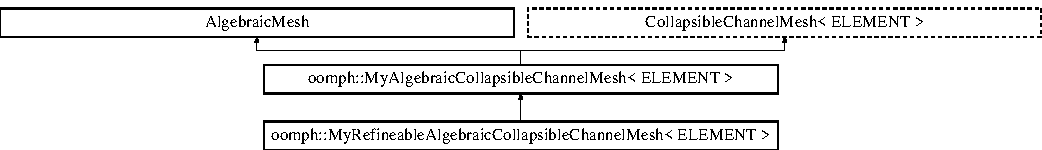
\includegraphics[height=2.009569cm]{classoomph_1_1MyAlgebraicCollapsibleChannelMesh}
\end{center}
\end{figure}
\subsection*{Public Member Functions}
\begin{DoxyCompactItemize}
\item 
\hyperlink{classoomph_1_1MyAlgebraicCollapsibleChannelMesh_a1a77973034fec46c16a41d1f4d250b0a}{My\+Algebraic\+Collapsible\+Channel\+Mesh} (const unsigned \&nup, const unsigned \&ncollapsible, const unsigned \&ndown, const unsigned \&ny, const double \&lup, const double \&lcollapsible, const double \&ldown, const double \&ly, Geom\+Object $\ast$wall\+\_\+pt, Time\+Stepper $\ast$time\+\_\+stepper\+\_\+pt=\&Mesh\+::\+Default\+\_\+\+Time\+Stepper)
\begin{DoxyCompactList}\small\item\em Constructor\+: Pass number of elements in upstream/collapsible/ downstream segment and across the channel; lengths of upstream/ collapsible/downstream segments and width of channel, pointer to Geom\+Object that defines the collapsible segment, and pointer to Time\+Stepper (defaults to the default timestepper, Steady). \end{DoxyCompactList}\item 
\hyperlink{classoomph_1_1MyAlgebraicCollapsibleChannelMesh_a36eed7b6be90d44726091c6d97d53e3f}{My\+Algebraic\+Collapsible\+Channel\+Mesh} (const unsigned \&nup, const unsigned \&ncollapsible, const unsigned \&ndown, const unsigned \&ny, const double \&lup, const double \&lcollapsible, const double \&ldown, const double \&ly, Geom\+Object $\ast$wall\+\_\+pt, Collapsible\+Channel\+Domain\+::\+B\+L\+Squash\+Fct\+Pt bl\+\_\+squash\+\_\+function\+\_\+pt, Time\+Stepper $\ast$time\+\_\+stepper\+\_\+pt=\&Mesh\+::\+Default\+\_\+\+Time\+Stepper)
\begin{DoxyCompactList}\small\item\em Constructor\+: Pass number of elements in upstream/collapsible/ downstream segment and across the channel; lengths of upstream/ collapsible/downstream segments and width of channel, pointer to Geom\+Object that defines the collapsible segment, function pointer to \char`\"{}boundary layer squash function\char`\"{}, and pointer to Time\+Stepper (defaults to the default timestepper, Steady). \end{DoxyCompactList}\item 
virtual \hyperlink{classoomph_1_1MyAlgebraicCollapsibleChannelMesh_aba200b3263e6a11eb26739965df8cbcc}{$\sim$\+My\+Algebraic\+Collapsible\+Channel\+Mesh} ()
\begin{DoxyCompactList}\small\item\em Destructor\+: empty. \end{DoxyCompactList}\item 
Collapsible\+Channel\+Domain\+::\+B\+L\+Squash\+Fct\+Pt \& \hyperlink{classoomph_1_1MyAlgebraicCollapsibleChannelMesh_ad488fafa275b664c739828d3e2a281bf}{bl\+\_\+squash\+\_\+fct\+\_\+pt} ()
\begin{DoxyCompactList}\small\item\em Function pointer for function that squashes the mesh near the walls. Default trivial mapping (the identity) leaves vertical nodal positions unchanged. Mapping is used in underlying Collapsible\+Channel\+Domain. This (deliberately broken) function overloads the one in the Collapsible\+Channel\+Mesh base class. \end{DoxyCompactList}\item 
void \hyperlink{classoomph_1_1MyAlgebraicCollapsibleChannelMesh_a28702ba4f4f10e9dfc495c916ddf6f82}{algebraic\+\_\+node\+\_\+update} (const unsigned \&t, Algebraic\+Node $\ast$\&node\+\_\+pt)
\begin{DoxyCompactList}\small\item\em Update nodal position at time level t (t=0\+: present; t$>$0\+: previous) \end{DoxyCompactList}\item 
void \hyperlink{classoomph_1_1MyAlgebraicCollapsibleChannelMesh_adb6c8c672e0810b59174babf3623f5bd}{update\+\_\+node\+\_\+update} (Algebraic\+Node $\ast$\&node\+\_\+pt)
\begin{DoxyCompactList}\small\item\em Update the geometric references that are used to update node after mesh adaptation. Empty -- no update of node update required. \end{DoxyCompactList}\end{DoxyCompactItemize}
\subsection*{Protected Member Functions}
\begin{DoxyCompactItemize}
\item 
void \hyperlink{classoomph_1_1MyAlgebraicCollapsibleChannelMesh_ad5ae1032e856e8997cc138b84a089452}{setup\+\_\+algebraic\+\_\+node\+\_\+update} ()
\begin{DoxyCompactList}\small\item\em Function to setup the algebraic node update. \end{DoxyCompactList}\end{DoxyCompactItemize}
\subsection*{Protected Attributes}
\begin{DoxyCompactItemize}
\item 
Collapsible\+Channel\+Domain\+::\+B\+L\+Squash\+Fct\+Pt \hyperlink{classoomph_1_1MyAlgebraicCollapsibleChannelMesh_ad60e33d1b61229a7d591bd963713aa03}{Dummy\+\_\+fct\+\_\+pt}
\begin{DoxyCompactList}\small\item\em Dummy function pointer. \end{DoxyCompactList}\end{DoxyCompactItemize}


\subsection{Detailed Description}
\subsubsection*{template$<$class E\+L\+E\+M\+E\+NT$>$\newline
class oomph\+::\+My\+Algebraic\+Collapsible\+Channel\+Mesh$<$ E\+L\+E\+M\+E\+N\+T $>$}

Collapsible channel mesh with algebraic node update. 

Definition at line 52 of file my\+\_\+alg\+\_\+channel\+\_\+mesh.\+h.



\subsection{Constructor \& Destructor Documentation}
\mbox{\Hypertarget{classoomph_1_1MyAlgebraicCollapsibleChannelMesh_a1a77973034fec46c16a41d1f4d250b0a}\label{classoomph_1_1MyAlgebraicCollapsibleChannelMesh_a1a77973034fec46c16a41d1f4d250b0a}} 
\index{oomph\+::\+My\+Algebraic\+Collapsible\+Channel\+Mesh@{oomph\+::\+My\+Algebraic\+Collapsible\+Channel\+Mesh}!My\+Algebraic\+Collapsible\+Channel\+Mesh@{My\+Algebraic\+Collapsible\+Channel\+Mesh}}
\index{My\+Algebraic\+Collapsible\+Channel\+Mesh@{My\+Algebraic\+Collapsible\+Channel\+Mesh}!oomph\+::\+My\+Algebraic\+Collapsible\+Channel\+Mesh@{oomph\+::\+My\+Algebraic\+Collapsible\+Channel\+Mesh}}
\subsubsection{\texorpdfstring{My\+Algebraic\+Collapsible\+Channel\+Mesh()}{MyAlgebraicCollapsibleChannelMesh()}\hspace{0.1cm}{\footnotesize\ttfamily [1/2]}}
{\footnotesize\ttfamily template$<$class E\+L\+E\+M\+E\+NT$>$ \\
\hyperlink{classoomph_1_1MyAlgebraicCollapsibleChannelMesh}{oomph\+::\+My\+Algebraic\+Collapsible\+Channel\+Mesh}$<$ E\+L\+E\+M\+E\+NT $>$\+::\hyperlink{classoomph_1_1MyAlgebraicCollapsibleChannelMesh}{My\+Algebraic\+Collapsible\+Channel\+Mesh} (\begin{DoxyParamCaption}\item[{const unsigned \&}]{nup,  }\item[{const unsigned \&}]{ncollapsible,  }\item[{const unsigned \&}]{ndown,  }\item[{const unsigned \&}]{ny,  }\item[{const double \&}]{lup,  }\item[{const double \&}]{lcollapsible,  }\item[{const double \&}]{ldown,  }\item[{const double \&}]{ly,  }\item[{Geom\+Object $\ast$}]{wall\+\_\+pt,  }\item[{Time\+Stepper $\ast$}]{time\+\_\+stepper\+\_\+pt = {\ttfamily \&Mesh\+:\+:Default\+\_\+TimeStepper} }\end{DoxyParamCaption})\hspace{0.3cm}{\ttfamily [inline]}}



Constructor\+: Pass number of elements in upstream/collapsible/ downstream segment and across the channel; lengths of upstream/ collapsible/downstream segments and width of channel, pointer to Geom\+Object that defines the collapsible segment, and pointer to Time\+Stepper (defaults to the default timestepper, Steady). 



Definition at line 64 of file my\+\_\+alg\+\_\+channel\+\_\+mesh.\+h.



References oomph\+::\+My\+Algebraic\+Collapsible\+Channel\+Mesh$<$ E\+L\+E\+M\+E\+N\+T $>$\+::setup\+\_\+algebraic\+\_\+node\+\_\+update().

\mbox{\Hypertarget{classoomph_1_1MyAlgebraicCollapsibleChannelMesh_a36eed7b6be90d44726091c6d97d53e3f}\label{classoomph_1_1MyAlgebraicCollapsibleChannelMesh_a36eed7b6be90d44726091c6d97d53e3f}} 
\index{oomph\+::\+My\+Algebraic\+Collapsible\+Channel\+Mesh@{oomph\+::\+My\+Algebraic\+Collapsible\+Channel\+Mesh}!My\+Algebraic\+Collapsible\+Channel\+Mesh@{My\+Algebraic\+Collapsible\+Channel\+Mesh}}
\index{My\+Algebraic\+Collapsible\+Channel\+Mesh@{My\+Algebraic\+Collapsible\+Channel\+Mesh}!oomph\+::\+My\+Algebraic\+Collapsible\+Channel\+Mesh@{oomph\+::\+My\+Algebraic\+Collapsible\+Channel\+Mesh}}
\subsubsection{\texorpdfstring{My\+Algebraic\+Collapsible\+Channel\+Mesh()}{MyAlgebraicCollapsibleChannelMesh()}\hspace{0.1cm}{\footnotesize\ttfamily [2/2]}}
{\footnotesize\ttfamily template$<$class E\+L\+E\+M\+E\+NT$>$ \\
\hyperlink{classoomph_1_1MyAlgebraicCollapsibleChannelMesh}{oomph\+::\+My\+Algebraic\+Collapsible\+Channel\+Mesh}$<$ E\+L\+E\+M\+E\+NT $>$\+::\hyperlink{classoomph_1_1MyAlgebraicCollapsibleChannelMesh}{My\+Algebraic\+Collapsible\+Channel\+Mesh} (\begin{DoxyParamCaption}\item[{const unsigned \&}]{nup,  }\item[{const unsigned \&}]{ncollapsible,  }\item[{const unsigned \&}]{ndown,  }\item[{const unsigned \&}]{ny,  }\item[{const double \&}]{lup,  }\item[{const double \&}]{lcollapsible,  }\item[{const double \&}]{ldown,  }\item[{const double \&}]{ly,  }\item[{Geom\+Object $\ast$}]{wall\+\_\+pt,  }\item[{Collapsible\+Channel\+Domain\+::\+B\+L\+Squash\+Fct\+Pt}]{bl\+\_\+squash\+\_\+function\+\_\+pt,  }\item[{Time\+Stepper $\ast$}]{time\+\_\+stepper\+\_\+pt = {\ttfamily \&Mesh\+:\+:Default\+\_\+TimeStepper} }\end{DoxyParamCaption})\hspace{0.3cm}{\ttfamily [inline]}}



Constructor\+: Pass number of elements in upstream/collapsible/ downstream segment and across the channel; lengths of upstream/ collapsible/downstream segments and width of channel, pointer to Geom\+Object that defines the collapsible segment, function pointer to \char`\"{}boundary layer squash function\char`\"{}, and pointer to Time\+Stepper (defaults to the default timestepper, Steady). 



Definition at line 92 of file my\+\_\+alg\+\_\+channel\+\_\+mesh.\+h.



References oomph\+::\+My\+Algebraic\+Collapsible\+Channel\+Mesh$<$ E\+L\+E\+M\+E\+N\+T $>$\+::setup\+\_\+algebraic\+\_\+node\+\_\+update().

\mbox{\Hypertarget{classoomph_1_1MyAlgebraicCollapsibleChannelMesh_aba200b3263e6a11eb26739965df8cbcc}\label{classoomph_1_1MyAlgebraicCollapsibleChannelMesh_aba200b3263e6a11eb26739965df8cbcc}} 
\index{oomph\+::\+My\+Algebraic\+Collapsible\+Channel\+Mesh@{oomph\+::\+My\+Algebraic\+Collapsible\+Channel\+Mesh}!````~My\+Algebraic\+Collapsible\+Channel\+Mesh@{$\sim$\+My\+Algebraic\+Collapsible\+Channel\+Mesh}}
\index{````~My\+Algebraic\+Collapsible\+Channel\+Mesh@{$\sim$\+My\+Algebraic\+Collapsible\+Channel\+Mesh}!oomph\+::\+My\+Algebraic\+Collapsible\+Channel\+Mesh@{oomph\+::\+My\+Algebraic\+Collapsible\+Channel\+Mesh}}
\subsubsection{\texorpdfstring{$\sim$\+My\+Algebraic\+Collapsible\+Channel\+Mesh()}{~MyAlgebraicCollapsibleChannelMesh()}}
{\footnotesize\ttfamily template$<$class E\+L\+E\+M\+E\+NT$>$ \\
virtual \hyperlink{classoomph_1_1MyAlgebraicCollapsibleChannelMesh}{oomph\+::\+My\+Algebraic\+Collapsible\+Channel\+Mesh}$<$ E\+L\+E\+M\+E\+NT $>$\+::$\sim$\hyperlink{classoomph_1_1MyAlgebraicCollapsibleChannelMesh}{My\+Algebraic\+Collapsible\+Channel\+Mesh} (\begin{DoxyParamCaption}{ }\end{DoxyParamCaption})\hspace{0.3cm}{\ttfamily [inline]}, {\ttfamily [virtual]}}



Destructor\+: empty. 



Definition at line 122 of file my\+\_\+alg\+\_\+channel\+\_\+mesh.\+h.



\subsection{Member Function Documentation}
\mbox{\Hypertarget{classoomph_1_1MyAlgebraicCollapsibleChannelMesh_a28702ba4f4f10e9dfc495c916ddf6f82}\label{classoomph_1_1MyAlgebraicCollapsibleChannelMesh_a28702ba4f4f10e9dfc495c916ddf6f82}} 
\index{oomph\+::\+My\+Algebraic\+Collapsible\+Channel\+Mesh@{oomph\+::\+My\+Algebraic\+Collapsible\+Channel\+Mesh}!algebraic\+\_\+node\+\_\+update@{algebraic\+\_\+node\+\_\+update}}
\index{algebraic\+\_\+node\+\_\+update@{algebraic\+\_\+node\+\_\+update}!oomph\+::\+My\+Algebraic\+Collapsible\+Channel\+Mesh@{oomph\+::\+My\+Algebraic\+Collapsible\+Channel\+Mesh}}
\subsubsection{\texorpdfstring{algebraic\+\_\+node\+\_\+update()}{algebraic\_node\_update()}}
{\footnotesize\ttfamily template$<$class E\+L\+E\+M\+E\+NT $>$ \\
void \hyperlink{classoomph_1_1MyAlgebraicCollapsibleChannelMesh}{oomph\+::\+My\+Algebraic\+Collapsible\+Channel\+Mesh}$<$ E\+L\+E\+M\+E\+NT $>$\+::algebraic\+\_\+node\+\_\+update (\begin{DoxyParamCaption}\item[{const unsigned \&}]{t,  }\item[{Algebraic\+Node $\ast$\&}]{node\+\_\+pt }\end{DoxyParamCaption})}



Update nodal position at time level t (t=0\+: present; t$>$0\+: previous) 

Perform algebraic mesh update at time level t (t=0\+: present; t$>$0\+: previous) 

Definition at line 359 of file my\+\_\+alg\+\_\+channel\+\_\+mesh.\+h.



Referenced by oomph\+::\+My\+Algebraic\+Collapsible\+Channel\+Mesh$<$ E\+L\+E\+M\+E\+N\+T $>$\+::bl\+\_\+squash\+\_\+fct\+\_\+pt().

\mbox{\Hypertarget{classoomph_1_1MyAlgebraicCollapsibleChannelMesh_ad488fafa275b664c739828d3e2a281bf}\label{classoomph_1_1MyAlgebraicCollapsibleChannelMesh_ad488fafa275b664c739828d3e2a281bf}} 
\index{oomph\+::\+My\+Algebraic\+Collapsible\+Channel\+Mesh@{oomph\+::\+My\+Algebraic\+Collapsible\+Channel\+Mesh}!bl\+\_\+squash\+\_\+fct\+\_\+pt@{bl\+\_\+squash\+\_\+fct\+\_\+pt}}
\index{bl\+\_\+squash\+\_\+fct\+\_\+pt@{bl\+\_\+squash\+\_\+fct\+\_\+pt}!oomph\+::\+My\+Algebraic\+Collapsible\+Channel\+Mesh@{oomph\+::\+My\+Algebraic\+Collapsible\+Channel\+Mesh}}
\subsubsection{\texorpdfstring{bl\+\_\+squash\+\_\+fct\+\_\+pt()}{bl\_squash\_fct\_pt()}}
{\footnotesize\ttfamily template$<$class E\+L\+E\+M\+E\+NT$>$ \\
Collapsible\+Channel\+Domain\+::\+B\+L\+Squash\+Fct\+Pt\& \hyperlink{classoomph_1_1MyAlgebraicCollapsibleChannelMesh}{oomph\+::\+My\+Algebraic\+Collapsible\+Channel\+Mesh}$<$ E\+L\+E\+M\+E\+NT $>$\+::bl\+\_\+squash\+\_\+fct\+\_\+pt (\begin{DoxyParamCaption}{ }\end{DoxyParamCaption})\hspace{0.3cm}{\ttfamily [inline]}}



Function pointer for function that squashes the mesh near the walls. Default trivial mapping (the identity) leaves vertical nodal positions unchanged. Mapping is used in underlying Collapsible\+Channel\+Domain. This (deliberately broken) function overloads the one in the Collapsible\+Channel\+Mesh base class. 



Definition at line 130 of file my\+\_\+alg\+\_\+channel\+\_\+mesh.\+h.



References oomph\+::\+My\+Algebraic\+Collapsible\+Channel\+Mesh$<$ E\+L\+E\+M\+E\+N\+T $>$\+::algebraic\+\_\+node\+\_\+update(), and oomph\+::\+My\+Algebraic\+Collapsible\+Channel\+Mesh$<$ E\+L\+E\+M\+E\+N\+T $>$\+::\+Dummy\+\_\+fct\+\_\+pt.

\mbox{\Hypertarget{classoomph_1_1MyAlgebraicCollapsibleChannelMesh_ad5ae1032e856e8997cc138b84a089452}\label{classoomph_1_1MyAlgebraicCollapsibleChannelMesh_ad5ae1032e856e8997cc138b84a089452}} 
\index{oomph\+::\+My\+Algebraic\+Collapsible\+Channel\+Mesh@{oomph\+::\+My\+Algebraic\+Collapsible\+Channel\+Mesh}!setup\+\_\+algebraic\+\_\+node\+\_\+update@{setup\+\_\+algebraic\+\_\+node\+\_\+update}}
\index{setup\+\_\+algebraic\+\_\+node\+\_\+update@{setup\+\_\+algebraic\+\_\+node\+\_\+update}!oomph\+::\+My\+Algebraic\+Collapsible\+Channel\+Mesh@{oomph\+::\+My\+Algebraic\+Collapsible\+Channel\+Mesh}}
\subsubsection{\texorpdfstring{setup\+\_\+algebraic\+\_\+node\+\_\+update()}{setup\_algebraic\_node\_update()}}
{\footnotesize\ttfamily template$<$class E\+L\+E\+M\+E\+NT $>$ \\
void \hyperlink{classoomph_1_1MyAlgebraicCollapsibleChannelMesh}{oomph\+::\+My\+Algebraic\+Collapsible\+Channel\+Mesh}$<$ E\+L\+E\+M\+E\+NT $>$\+::setup\+\_\+algebraic\+\_\+node\+\_\+update (\begin{DoxyParamCaption}{ }\end{DoxyParamCaption})\hspace{0.3cm}{\ttfamily [protected]}}



Function to setup the algebraic node update. 

Setup algebraic mesh update -- assumes that mesh has initially been set up with the wall in its undeformed position. 

Definition at line 272 of file my\+\_\+alg\+\_\+channel\+\_\+mesh.\+h.



Referenced by oomph\+::\+My\+Algebraic\+Collapsible\+Channel\+Mesh$<$ E\+L\+E\+M\+E\+N\+T $>$\+::\+My\+Algebraic\+Collapsible\+Channel\+Mesh(), and oomph\+::\+My\+Algebraic\+Collapsible\+Channel\+Mesh$<$ E\+L\+E\+M\+E\+N\+T $>$\+::update\+\_\+node\+\_\+update().

\mbox{\Hypertarget{classoomph_1_1MyAlgebraicCollapsibleChannelMesh_adb6c8c672e0810b59174babf3623f5bd}\label{classoomph_1_1MyAlgebraicCollapsibleChannelMesh_adb6c8c672e0810b59174babf3623f5bd}} 
\index{oomph\+::\+My\+Algebraic\+Collapsible\+Channel\+Mesh@{oomph\+::\+My\+Algebraic\+Collapsible\+Channel\+Mesh}!update\+\_\+node\+\_\+update@{update\+\_\+node\+\_\+update}}
\index{update\+\_\+node\+\_\+update@{update\+\_\+node\+\_\+update}!oomph\+::\+My\+Algebraic\+Collapsible\+Channel\+Mesh@{oomph\+::\+My\+Algebraic\+Collapsible\+Channel\+Mesh}}
\subsubsection{\texorpdfstring{update\+\_\+node\+\_\+update()}{update\_node\_update()}}
{\footnotesize\ttfamily template$<$class E\+L\+E\+M\+E\+NT$>$ \\
void \hyperlink{classoomph_1_1MyAlgebraicCollapsibleChannelMesh}{oomph\+::\+My\+Algebraic\+Collapsible\+Channel\+Mesh}$<$ E\+L\+E\+M\+E\+NT $>$\+::update\+\_\+node\+\_\+update (\begin{DoxyParamCaption}\item[{Algebraic\+Node $\ast$\&}]{node\+\_\+pt }\end{DoxyParamCaption})\hspace{0.3cm}{\ttfamily [inline]}}



Update the geometric references that are used to update node after mesh adaptation. Empty -- no update of node update required. 



Definition at line 156 of file my\+\_\+alg\+\_\+channel\+\_\+mesh.\+h.



References oomph\+::\+My\+Algebraic\+Collapsible\+Channel\+Mesh$<$ E\+L\+E\+M\+E\+N\+T $>$\+::setup\+\_\+algebraic\+\_\+node\+\_\+update().



\subsection{Member Data Documentation}
\mbox{\Hypertarget{classoomph_1_1MyAlgebraicCollapsibleChannelMesh_ad60e33d1b61229a7d591bd963713aa03}\label{classoomph_1_1MyAlgebraicCollapsibleChannelMesh_ad60e33d1b61229a7d591bd963713aa03}} 
\index{oomph\+::\+My\+Algebraic\+Collapsible\+Channel\+Mesh@{oomph\+::\+My\+Algebraic\+Collapsible\+Channel\+Mesh}!Dummy\+\_\+fct\+\_\+pt@{Dummy\+\_\+fct\+\_\+pt}}
\index{Dummy\+\_\+fct\+\_\+pt@{Dummy\+\_\+fct\+\_\+pt}!oomph\+::\+My\+Algebraic\+Collapsible\+Channel\+Mesh@{oomph\+::\+My\+Algebraic\+Collapsible\+Channel\+Mesh}}
\subsubsection{\texorpdfstring{Dummy\+\_\+fct\+\_\+pt}{Dummy\_fct\_pt}}
{\footnotesize\ttfamily template$<$class E\+L\+E\+M\+E\+NT$>$ \\
Collapsible\+Channel\+Domain\+::\+B\+L\+Squash\+Fct\+Pt \hyperlink{classoomph_1_1MyAlgebraicCollapsibleChannelMesh}{oomph\+::\+My\+Algebraic\+Collapsible\+Channel\+Mesh}$<$ E\+L\+E\+M\+E\+NT $>$\+::Dummy\+\_\+fct\+\_\+pt\hspace{0.3cm}{\ttfamily [protected]}}



Dummy function pointer. 



Definition at line 165 of file my\+\_\+alg\+\_\+channel\+\_\+mesh.\+h.



Referenced by oomph\+::\+My\+Algebraic\+Collapsible\+Channel\+Mesh$<$ E\+L\+E\+M\+E\+N\+T $>$\+::bl\+\_\+squash\+\_\+fct\+\_\+pt().



The documentation for this class was generated from the following file\+:\begin{DoxyCompactItemize}
\item 
\hyperlink{my__alg__channel__mesh_8h}{my\+\_\+alg\+\_\+channel\+\_\+mesh.\+h}\end{DoxyCompactItemize}

\hypertarget{classoomph_1_1MyRefineableAlgebraicCollapsibleChannelMesh}{}\section{oomph\+:\+:My\+Refineable\+Algebraic\+Collapsible\+Channel\+Mesh$<$ E\+L\+E\+M\+E\+NT $>$ Class Template Reference}
\label{classoomph_1_1MyRefineableAlgebraicCollapsibleChannelMesh}\index{oomph\+::\+My\+Refineable\+Algebraic\+Collapsible\+Channel\+Mesh$<$ E\+L\+E\+M\+E\+N\+T $>$@{oomph\+::\+My\+Refineable\+Algebraic\+Collapsible\+Channel\+Mesh$<$ E\+L\+E\+M\+E\+N\+T $>$}}


{\ttfamily \#include $<$my\+\_\+alg\+\_\+channel\+\_\+mesh.\+h$>$}

Inheritance diagram for oomph\+:\+:My\+Refineable\+Algebraic\+Collapsible\+Channel\+Mesh$<$ E\+L\+E\+M\+E\+NT $>$\+:\begin{figure}[H]
\begin{center}
\leavevmode
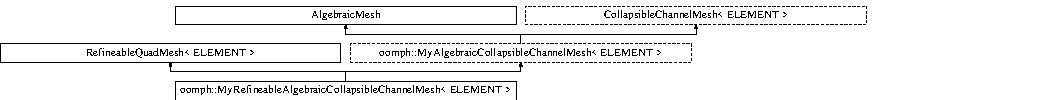
\includegraphics[height=1.339713cm]{classoomph_1_1MyRefineableAlgebraicCollapsibleChannelMesh}
\end{center}
\end{figure}
\subsection*{Public Member Functions}
\begin{DoxyCompactItemize}
\item 
\hyperlink{classoomph_1_1MyRefineableAlgebraicCollapsibleChannelMesh_a79a68cc8d0515711e03a3a6e67d8b10f}{My\+Refineable\+Algebraic\+Collapsible\+Channel\+Mesh} (const unsigned \&nup, const unsigned \&ncollapsible, const unsigned \&ndown, const unsigned \&ny, const double \&lup, const double \&lcollapsible, const double \&ldown, const double \&ly, Geom\+Object $\ast$wall\+\_\+pt, Time\+Stepper $\ast$time\+\_\+stepper\+\_\+pt=\&Mesh\+::\+Default\+\_\+\+Time\+Stepper)
\begin{DoxyCompactList}\small\item\em Constructor\+: Pass number of elements in upstream/collapsible/ downstream segment and across the channel; lengths of upstream/ collapsible/downstream segments and width of channel, pointer to Geom\+Object that defines the collapsible segment, function pointer to \char`\"{}boundary layer squash function\char`\"{}, and pointer to Time\+Stepper (defaults to the default timestepper, Steady). \end{DoxyCompactList}\item 
\hyperlink{classoomph_1_1MyRefineableAlgebraicCollapsibleChannelMesh_a1a733580c1e040c6d546e6ec78d844ee}{My\+Refineable\+Algebraic\+Collapsible\+Channel\+Mesh} (const unsigned \&nup, const unsigned \&ncollapsible, const unsigned \&ndown, const unsigned \&ny, const double \&lup, const double \&lcollapsible, const double \&ldown, const double \&ly, Geom\+Object $\ast$wall\+\_\+pt, Collapsible\+Channel\+Domain\+::\+B\+L\+Squash\+Fct\+Pt bl\+\_\+squash\+\_\+function\+\_\+pt, Time\+Stepper $\ast$time\+\_\+stepper\+\_\+pt=\&Mesh\+::\+Default\+\_\+\+Time\+Stepper)
\begin{DoxyCompactList}\small\item\em Constructor\+: Pass number of elements in upstream/collapsible/ downstream segment and across the channel; lengths of upstream/ collapsible/downstream segments and width of channel, pointer to Geom\+Object that defines the collapsible segment, function pointer to \char`\"{}boundary layer squash function\char`\"{}, and pointer to Time\+Stepper (defaults to the default timestepper, Steady). \end{DoxyCompactList}\end{DoxyCompactItemize}
\subsection*{Additional Inherited Members}


\subsection{Detailed Description}
\subsubsection*{template$<$class E\+L\+E\+M\+E\+NT$>$\newline
class oomph\+::\+My\+Refineable\+Algebraic\+Collapsible\+Channel\+Mesh$<$ E\+L\+E\+M\+E\+N\+T $>$}

Refineable version of the Collapsible\+Channel mesh with algebraic node update. 

Definition at line 184 of file my\+\_\+alg\+\_\+channel\+\_\+mesh.\+h.



\subsection{Constructor \& Destructor Documentation}
\mbox{\Hypertarget{classoomph_1_1MyRefineableAlgebraicCollapsibleChannelMesh_a79a68cc8d0515711e03a3a6e67d8b10f}\label{classoomph_1_1MyRefineableAlgebraicCollapsibleChannelMesh_a79a68cc8d0515711e03a3a6e67d8b10f}} 
\index{oomph\+::\+My\+Refineable\+Algebraic\+Collapsible\+Channel\+Mesh@{oomph\+::\+My\+Refineable\+Algebraic\+Collapsible\+Channel\+Mesh}!My\+Refineable\+Algebraic\+Collapsible\+Channel\+Mesh@{My\+Refineable\+Algebraic\+Collapsible\+Channel\+Mesh}}
\index{My\+Refineable\+Algebraic\+Collapsible\+Channel\+Mesh@{My\+Refineable\+Algebraic\+Collapsible\+Channel\+Mesh}!oomph\+::\+My\+Refineable\+Algebraic\+Collapsible\+Channel\+Mesh@{oomph\+::\+My\+Refineable\+Algebraic\+Collapsible\+Channel\+Mesh}}
\subsubsection{\texorpdfstring{My\+Refineable\+Algebraic\+Collapsible\+Channel\+Mesh()}{MyRefineableAlgebraicCollapsibleChannelMesh()}\hspace{0.1cm}{\footnotesize\ttfamily [1/2]}}
{\footnotesize\ttfamily template$<$class E\+L\+E\+M\+E\+NT$>$ \\
\hyperlink{classoomph_1_1MyRefineableAlgebraicCollapsibleChannelMesh}{oomph\+::\+My\+Refineable\+Algebraic\+Collapsible\+Channel\+Mesh}$<$ E\+L\+E\+M\+E\+NT $>$\+::\hyperlink{classoomph_1_1MyRefineableAlgebraicCollapsibleChannelMesh}{My\+Refineable\+Algebraic\+Collapsible\+Channel\+Mesh} (\begin{DoxyParamCaption}\item[{const unsigned \&}]{nup,  }\item[{const unsigned \&}]{ncollapsible,  }\item[{const unsigned \&}]{ndown,  }\item[{const unsigned \&}]{ny,  }\item[{const double \&}]{lup,  }\item[{const double \&}]{lcollapsible,  }\item[{const double \&}]{ldown,  }\item[{const double \&}]{ly,  }\item[{Geom\+Object $\ast$}]{wall\+\_\+pt,  }\item[{Time\+Stepper $\ast$}]{time\+\_\+stepper\+\_\+pt = {\ttfamily \&Mesh\+:\+:Default\+\_\+TimeStepper} }\end{DoxyParamCaption})\hspace{0.3cm}{\ttfamily [inline]}}



Constructor\+: Pass number of elements in upstream/collapsible/ downstream segment and across the channel; lengths of upstream/ collapsible/downstream segments and width of channel, pointer to Geom\+Object that defines the collapsible segment, function pointer to \char`\"{}boundary layer squash function\char`\"{}, and pointer to Time\+Stepper (defaults to the default timestepper, Steady). 



Definition at line 198 of file my\+\_\+alg\+\_\+channel\+\_\+mesh.\+h.

\mbox{\Hypertarget{classoomph_1_1MyRefineableAlgebraicCollapsibleChannelMesh_a1a733580c1e040c6d546e6ec78d844ee}\label{classoomph_1_1MyRefineableAlgebraicCollapsibleChannelMesh_a1a733580c1e040c6d546e6ec78d844ee}} 
\index{oomph\+::\+My\+Refineable\+Algebraic\+Collapsible\+Channel\+Mesh@{oomph\+::\+My\+Refineable\+Algebraic\+Collapsible\+Channel\+Mesh}!My\+Refineable\+Algebraic\+Collapsible\+Channel\+Mesh@{My\+Refineable\+Algebraic\+Collapsible\+Channel\+Mesh}}
\index{My\+Refineable\+Algebraic\+Collapsible\+Channel\+Mesh@{My\+Refineable\+Algebraic\+Collapsible\+Channel\+Mesh}!oomph\+::\+My\+Refineable\+Algebraic\+Collapsible\+Channel\+Mesh@{oomph\+::\+My\+Refineable\+Algebraic\+Collapsible\+Channel\+Mesh}}
\subsubsection{\texorpdfstring{My\+Refineable\+Algebraic\+Collapsible\+Channel\+Mesh()}{MyRefineableAlgebraicCollapsibleChannelMesh()}\hspace{0.1cm}{\footnotesize\ttfamily [2/2]}}
{\footnotesize\ttfamily template$<$class E\+L\+E\+M\+E\+NT$>$ \\
\hyperlink{classoomph_1_1MyRefineableAlgebraicCollapsibleChannelMesh}{oomph\+::\+My\+Refineable\+Algebraic\+Collapsible\+Channel\+Mesh}$<$ E\+L\+E\+M\+E\+NT $>$\+::\hyperlink{classoomph_1_1MyRefineableAlgebraicCollapsibleChannelMesh}{My\+Refineable\+Algebraic\+Collapsible\+Channel\+Mesh} (\begin{DoxyParamCaption}\item[{const unsigned \&}]{nup,  }\item[{const unsigned \&}]{ncollapsible,  }\item[{const unsigned \&}]{ndown,  }\item[{const unsigned \&}]{ny,  }\item[{const double \&}]{lup,  }\item[{const double \&}]{lcollapsible,  }\item[{const double \&}]{ldown,  }\item[{const double \&}]{ly,  }\item[{Geom\+Object $\ast$}]{wall\+\_\+pt,  }\item[{Collapsible\+Channel\+Domain\+::\+B\+L\+Squash\+Fct\+Pt}]{bl\+\_\+squash\+\_\+function\+\_\+pt,  }\item[{Time\+Stepper $\ast$}]{time\+\_\+stepper\+\_\+pt = {\ttfamily \&Mesh\+:\+:Default\+\_\+TimeStepper} }\end{DoxyParamCaption})\hspace{0.3cm}{\ttfamily [inline]}}



Constructor\+: Pass number of elements in upstream/collapsible/ downstream segment and across the channel; lengths of upstream/ collapsible/downstream segments and width of channel, pointer to Geom\+Object that defines the collapsible segment, function pointer to \char`\"{}boundary layer squash function\char`\"{}, and pointer to Time\+Stepper (defaults to the default timestepper, Steady). 



Definition at line 231 of file my\+\_\+alg\+\_\+channel\+\_\+mesh.\+h.



The documentation for this class was generated from the following file\+:\begin{DoxyCompactItemize}
\item 
\hyperlink{my__alg__channel__mesh_8h}{my\+\_\+alg\+\_\+channel\+\_\+mesh.\+h}\end{DoxyCompactItemize}

\hypertarget{classOscillatingWall}{}\section{Oscillating\+Wall Class Reference}
\label{classOscillatingWall}\index{Oscillating\+Wall@{Oscillating\+Wall}}
Inheritance diagram for Oscillating\+Wall\+:\begin{figure}[H]
\begin{center}
\leavevmode
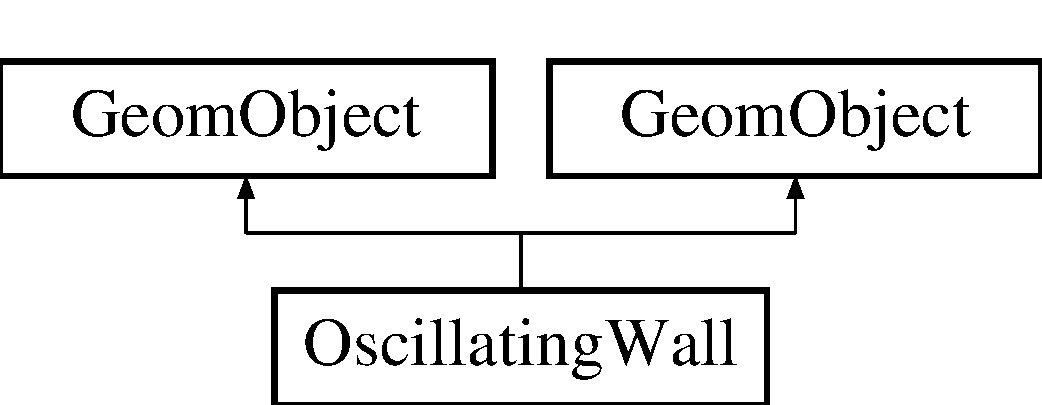
\includegraphics[height=2.000000cm]{classOscillatingWall}
\end{center}
\end{figure}
\subsection*{Public Member Functions}
\begin{DoxyCompactItemize}
\item 
\hyperlink{classOscillatingWall_a5ededc3d27eef5c4ef7e82ac5cdf6ff9}{Oscillating\+Wall} (const double \&h, const double \&x\+\_\+left, const double \&l, const double \&a, const double \&\hyperlink{classOscillatingWall_ac3e0098c026e23dd8be8ea29f6a9c101}{period}, Time $\ast$time\+\_\+pt)
\begin{DoxyCompactList}\small\item\em Constructor \+: It\textquotesingle{}s a 2D object, parametrised by one Lagrangian coordinate. Arguments\+: height at ends, x-\/coordinate of left end, length, amplitude of deflection, period of oscillation, and pointer to time object. \end{DoxyCompactList}\item 
\hyperlink{classOscillatingWall_adc35b40bdd733a244d6399d91fa20ade}{$\sim$\+Oscillating\+Wall} ()
\begin{DoxyCompactList}\small\item\em Destructor\+: Empty. \end{DoxyCompactList}\item 
double \& \hyperlink{classOscillatingWall_ae923c6a7abefe33efaf47a4b69d1b621}{amplitude} ()
\begin{DoxyCompactList}\small\item\em Access function to the amplitude. \end{DoxyCompactList}\item 
double \& \hyperlink{classOscillatingWall_ac3e0098c026e23dd8be8ea29f6a9c101}{period} ()
\begin{DoxyCompactList}\small\item\em Access function to the period. \end{DoxyCompactList}\item 
void \hyperlink{classOscillatingWall_abb4ae7e556479d2980a56963bd8d4558}{position} (const unsigned \&t, const Vector$<$ double $>$ \&zeta, Vector$<$ double $>$ \&r) const
\begin{DoxyCompactList}\small\item\em Position vector at Lagrangian coordinate zeta at time level t. \end{DoxyCompactList}\item 
void \hyperlink{classOscillatingWall_a5fce6728f975003d9e85f64c18ba7f55}{position} (const Vector$<$ double $>$ \&zeta, Vector$<$ double $>$ \&r) const
\begin{DoxyCompactList}\small\item\em \char`\"{}\+Current\char`\"{} position vector at Lagrangian coordinate zeta \end{DoxyCompactList}\item 
unsigned \hyperlink{classOscillatingWall_ae3fa3ef50ef7e082b255ba8125373581}{ngeom\+\_\+data} () const
\begin{DoxyCompactList}\small\item\em Number of geometric Data in Geom\+Object\+: None. \end{DoxyCompactList}\item 
\hyperlink{classOscillatingWall_a5ededc3d27eef5c4ef7e82ac5cdf6ff9}{Oscillating\+Wall} (const double \&h, const double \&x\+\_\+left, const double \&l, const double \&a, const double \&\hyperlink{classOscillatingWall_ac3e0098c026e23dd8be8ea29f6a9c101}{period}, Time $\ast$time\+\_\+pt)
\begin{DoxyCompactList}\small\item\em Constructor \+: It\textquotesingle{}s a 2D object, parametrised by one Lagrangian coordinate. Arguments\+: height at ends, x-\/coordinate of left end, length, amplitude of deflection, period of oscillation, and pointer to time object. \end{DoxyCompactList}\item 
\hyperlink{classOscillatingWall_adc35b40bdd733a244d6399d91fa20ade}{$\sim$\+Oscillating\+Wall} ()
\begin{DoxyCompactList}\small\item\em Destructor\+: Empty. \end{DoxyCompactList}\item 
double \& \hyperlink{classOscillatingWall_ae923c6a7abefe33efaf47a4b69d1b621}{amplitude} ()
\begin{DoxyCompactList}\small\item\em Access function to the amplitude. \end{DoxyCompactList}\item 
double \& \hyperlink{classOscillatingWall_ac3e0098c026e23dd8be8ea29f6a9c101}{period} ()
\begin{DoxyCompactList}\small\item\em Access function to the period. \end{DoxyCompactList}\item 
void \hyperlink{classOscillatingWall_abb4ae7e556479d2980a56963bd8d4558}{position} (const unsigned \&t, const Vector$<$ double $>$ \&zeta, Vector$<$ double $>$ \&r) const
\begin{DoxyCompactList}\small\item\em Position vector at Lagrangian coordinate zeta at time level t. \end{DoxyCompactList}\item 
void \hyperlink{classOscillatingWall_a5fce6728f975003d9e85f64c18ba7f55}{position} (const Vector$<$ double $>$ \&zeta, Vector$<$ double $>$ \&r) const
\begin{DoxyCompactList}\small\item\em \char`\"{}\+Current\char`\"{} position vector at Lagrangian coordinate zeta \end{DoxyCompactList}\item 
unsigned \hyperlink{classOscillatingWall_ae3fa3ef50ef7e082b255ba8125373581}{ngeom\+\_\+data} () const
\begin{DoxyCompactList}\small\item\em Number of geometric Data in Geom\+Object\+: None. \end{DoxyCompactList}\end{DoxyCompactItemize}
\subsection*{Private Attributes}
\begin{DoxyCompactItemize}
\item 
double \hyperlink{classOscillatingWall_aa587e944cac9e501e6d3323731145b95}{H}
\begin{DoxyCompactList}\small\item\em Height at ends. \end{DoxyCompactList}\item 
double \hyperlink{classOscillatingWall_ac5e2ad6d5ef2992ba9295118787190e6}{Length}
\begin{DoxyCompactList}\small\item\em Length. \end{DoxyCompactList}\item 
double \hyperlink{classOscillatingWall_a71a60ee3294746875a24aeeffb38f7ec}{X\+\_\+left}
\begin{DoxyCompactList}\small\item\em x-\/coordinate of left end \end{DoxyCompactList}\item 
double \hyperlink{classOscillatingWall_ac22b6ac70a42850ddbe2e9c4c16f4664}{A}
\begin{DoxyCompactList}\small\item\em Amplitude of oscillation. \end{DoxyCompactList}\item 
double \hyperlink{classOscillatingWall_a9db810649987a2011c7fe14d10b98b9a}{B}
\begin{DoxyCompactList}\small\item\em Relative amplitude of horizontal wall motion. \end{DoxyCompactList}\item 
double \hyperlink{classOscillatingWall_af33b31988c823d33a3b147281ec94599}{T}
\begin{DoxyCompactList}\small\item\em Period of the oscillations. \end{DoxyCompactList}\item 
Time $\ast$ \hyperlink{classOscillatingWall_a9c4bea6ec6e80ba23139cd5a1d4d25d5}{Time\+\_\+pt}
\begin{DoxyCompactList}\small\item\em Pointer to the global time object. \end{DoxyCompactList}\end{DoxyCompactItemize}


\subsection{Detailed Description}
Straight, horizontal channel wall at $ y=H $ deforms into an oscillating parabola. The amplitude of the oscillation $ A $ and its period is $ T $. The position vector to a point on the wall, parametrised by the Lagrangian coordinate $ \zeta \in [0,L]$, is therefore given by \[ {\bf R}(\zeta,t) = \left( \begin{array}{c} L_{up} + \zeta \\ 1 \end{array} \right) + A \left( \begin{array}{l} - B \sin\left(\frac{2\pi}{L_{collapsible}}\zeta\right) \\ \left( \frac{2}{L_{collapsible}}\right)^2 \zeta \ (L-\zeta) \end{array} \right) \ \sin\left(\frac{2\pi t}{T}\right) \ {\cal R}(t) \] The parameter $ B $ is zero by default. If it is set to a nonzero value, the material particles on the wall also perform some horizontal motion. The \char`\"{}ramp\char`\"{} function \[ {\cal R}(t) = \left\{ \begin{array}{ll} \frac{1}{2}(1-\cos(\pi t/T)) & \mbox{for $t<T$} \\ 1 & \mbox{for $t \ge T$} \end{array} \right. \] provides a \char`\"{}smooth\char`\"{} startup of the oscillation.

Straight, horizontal channel wall at $ y=H $ deforms into an oscillating parabola. The amplitude of the oscillation $ A $ and its period is $ T $. The position vector to a point on the wall, parametrised by the Lagrangian coordinate $ \zeta \in [0,L]$, is therefore given by \[ {\bf R}(\zeta,t) = \left( \begin{array}{c} L_{up} + \zeta \newline 1 \end{array} \right) + A \left( \begin{array}{l} - B \sin\left(\frac{2\pi}{L_{collapsible}}\zeta\right) \newline \left(\frac{2}{L_{collapsible}}\right)^2 \zeta \ (L-\zeta) \end{array} \right) \ \sin\left(\frac{2\pi t}{T}\right) \ {\cal R}(t) \] The parameter $ B $ is zero by default. If it is set to a nonzero value, the material particles on the wall also perform some horizontal motion. The \char`\"{}ramp\char`\"{} function \[ {\cal R}(t) = \left\{ \begin{array}{ll} \frac{1}{2}(1-\cos(\pi t/T)) & \mbox{for $t<T$} \\ 1 & \mbox{for $t \ge T$} \end{array} \right. \] provides a \char`\"{}smooth\char`\"{} startup of the oscillation. 

Definition at line 120 of file collapsible\+\_\+channel.\+cc.



\subsection{Constructor \& Destructor Documentation}
\mbox{\Hypertarget{classOscillatingWall_a5ededc3d27eef5c4ef7e82ac5cdf6ff9}\label{classOscillatingWall_a5ededc3d27eef5c4ef7e82ac5cdf6ff9}} 
\index{Oscillating\+Wall@{Oscillating\+Wall}!Oscillating\+Wall@{Oscillating\+Wall}}
\index{Oscillating\+Wall@{Oscillating\+Wall}!Oscillating\+Wall@{Oscillating\+Wall}}
\subsubsection{\texorpdfstring{Oscillating\+Wall()}{OscillatingWall()}\hspace{0.1cm}{\footnotesize\ttfamily [1/2]}}
{\footnotesize\ttfamily Oscillating\+Wall\+::\+Oscillating\+Wall (\begin{DoxyParamCaption}\item[{const double \&}]{h,  }\item[{const double \&}]{x\+\_\+left,  }\item[{const double \&}]{l,  }\item[{const double \&}]{a,  }\item[{const double \&}]{period,  }\item[{Time $\ast$}]{time\+\_\+pt }\end{DoxyParamCaption})\hspace{0.3cm}{\ttfamily [inline]}}



Constructor \+: It\textquotesingle{}s a 2D object, parametrised by one Lagrangian coordinate. Arguments\+: height at ends, x-\/coordinate of left end, length, amplitude of deflection, period of oscillation, and pointer to time object. 



Definition at line 129 of file collapsible\+\_\+channel.\+cc.

\mbox{\Hypertarget{classOscillatingWall_adc35b40bdd733a244d6399d91fa20ade}\label{classOscillatingWall_adc35b40bdd733a244d6399d91fa20ade}} 
\index{Oscillating\+Wall@{Oscillating\+Wall}!````~Oscillating\+Wall@{$\sim$\+Oscillating\+Wall}}
\index{````~Oscillating\+Wall@{$\sim$\+Oscillating\+Wall}!Oscillating\+Wall@{Oscillating\+Wall}}
\subsubsection{\texorpdfstring{$\sim$\+Oscillating\+Wall()}{~OscillatingWall()}\hspace{0.1cm}{\footnotesize\ttfamily [1/2]}}
{\footnotesize\ttfamily Oscillating\+Wall\+::$\sim$\+Oscillating\+Wall (\begin{DoxyParamCaption}{ }\end{DoxyParamCaption})\hspace{0.3cm}{\ttfamily [inline]}}



Destructor\+: Empty. 



Definition at line 136 of file collapsible\+\_\+channel.\+cc.

\mbox{\Hypertarget{classOscillatingWall_a5ededc3d27eef5c4ef7e82ac5cdf6ff9}\label{classOscillatingWall_a5ededc3d27eef5c4ef7e82ac5cdf6ff9}} 
\index{Oscillating\+Wall@{Oscillating\+Wall}!Oscillating\+Wall@{Oscillating\+Wall}}
\index{Oscillating\+Wall@{Oscillating\+Wall}!Oscillating\+Wall@{Oscillating\+Wall}}
\subsubsection{\texorpdfstring{Oscillating\+Wall()}{OscillatingWall()}\hspace{0.1cm}{\footnotesize\ttfamily [2/2]}}
{\footnotesize\ttfamily Oscillating\+Wall\+::\+Oscillating\+Wall (\begin{DoxyParamCaption}\item[{const double \&}]{h,  }\item[{const double \&}]{x\+\_\+left,  }\item[{const double \&}]{l,  }\item[{const double \&}]{a,  }\item[{const double \&}]{period,  }\item[{Time $\ast$}]{time\+\_\+pt }\end{DoxyParamCaption})\hspace{0.3cm}{\ttfamily [inline]}}



Constructor \+: It\textquotesingle{}s a 2D object, parametrised by one Lagrangian coordinate. Arguments\+: height at ends, x-\/coordinate of left end, length, amplitude of deflection, period of oscillation, and pointer to time object. 



Definition at line 130 of file collapsible\+\_\+channel\+\_\+algebraic.\+cc.

\mbox{\Hypertarget{classOscillatingWall_adc35b40bdd733a244d6399d91fa20ade}\label{classOscillatingWall_adc35b40bdd733a244d6399d91fa20ade}} 
\index{Oscillating\+Wall@{Oscillating\+Wall}!````~Oscillating\+Wall@{$\sim$\+Oscillating\+Wall}}
\index{````~Oscillating\+Wall@{$\sim$\+Oscillating\+Wall}!Oscillating\+Wall@{Oscillating\+Wall}}
\subsubsection{\texorpdfstring{$\sim$\+Oscillating\+Wall()}{~OscillatingWall()}\hspace{0.1cm}{\footnotesize\ttfamily [2/2]}}
{\footnotesize\ttfamily Oscillating\+Wall\+::$\sim$\+Oscillating\+Wall (\begin{DoxyParamCaption}{ }\end{DoxyParamCaption})\hspace{0.3cm}{\ttfamily [inline]}}



Destructor\+: Empty. 



Definition at line 137 of file collapsible\+\_\+channel\+\_\+algebraic.\+cc.



\subsection{Member Function Documentation}
\mbox{\Hypertarget{classOscillatingWall_ae923c6a7abefe33efaf47a4b69d1b621}\label{classOscillatingWall_ae923c6a7abefe33efaf47a4b69d1b621}} 
\index{Oscillating\+Wall@{Oscillating\+Wall}!amplitude@{amplitude}}
\index{amplitude@{amplitude}!Oscillating\+Wall@{Oscillating\+Wall}}
\subsubsection{\texorpdfstring{amplitude()}{amplitude()}\hspace{0.1cm}{\footnotesize\ttfamily [1/2]}}
{\footnotesize\ttfamily double\& Oscillating\+Wall\+::amplitude (\begin{DoxyParamCaption}{ }\end{DoxyParamCaption})\hspace{0.3cm}{\ttfamily [inline]}}



Access function to the amplitude. 



Definition at line 139 of file collapsible\+\_\+channel.\+cc.

\mbox{\Hypertarget{classOscillatingWall_ae923c6a7abefe33efaf47a4b69d1b621}\label{classOscillatingWall_ae923c6a7abefe33efaf47a4b69d1b621}} 
\index{Oscillating\+Wall@{Oscillating\+Wall}!amplitude@{amplitude}}
\index{amplitude@{amplitude}!Oscillating\+Wall@{Oscillating\+Wall}}
\subsubsection{\texorpdfstring{amplitude()}{amplitude()}\hspace{0.1cm}{\footnotesize\ttfamily [2/2]}}
{\footnotesize\ttfamily double\& Oscillating\+Wall\+::amplitude (\begin{DoxyParamCaption}{ }\end{DoxyParamCaption})\hspace{0.3cm}{\ttfamily [inline]}}



Access function to the amplitude. 



Definition at line 140 of file collapsible\+\_\+channel\+\_\+algebraic.\+cc.

\mbox{\Hypertarget{classOscillatingWall_ae3fa3ef50ef7e082b255ba8125373581}\label{classOscillatingWall_ae3fa3ef50ef7e082b255ba8125373581}} 
\index{Oscillating\+Wall@{Oscillating\+Wall}!ngeom\+\_\+data@{ngeom\+\_\+data}}
\index{ngeom\+\_\+data@{ngeom\+\_\+data}!Oscillating\+Wall@{Oscillating\+Wall}}
\subsubsection{\texorpdfstring{ngeom\+\_\+data()}{ngeom\_data()}\hspace{0.1cm}{\footnotesize\ttfamily [1/2]}}
{\footnotesize\ttfamily unsigned Oscillating\+Wall\+::ngeom\+\_\+data (\begin{DoxyParamCaption}{ }\end{DoxyParamCaption}) const\hspace{0.3cm}{\ttfamily [inline]}}



Number of geometric Data in Geom\+Object\+: None. 



Definition at line 176 of file collapsible\+\_\+channel.\+cc.

\mbox{\Hypertarget{classOscillatingWall_ae3fa3ef50ef7e082b255ba8125373581}\label{classOscillatingWall_ae3fa3ef50ef7e082b255ba8125373581}} 
\index{Oscillating\+Wall@{Oscillating\+Wall}!ngeom\+\_\+data@{ngeom\+\_\+data}}
\index{ngeom\+\_\+data@{ngeom\+\_\+data}!Oscillating\+Wall@{Oscillating\+Wall}}
\subsubsection{\texorpdfstring{ngeom\+\_\+data()}{ngeom\_data()}\hspace{0.1cm}{\footnotesize\ttfamily [2/2]}}
{\footnotesize\ttfamily unsigned Oscillating\+Wall\+::ngeom\+\_\+data (\begin{DoxyParamCaption}{ }\end{DoxyParamCaption}) const\hspace{0.3cm}{\ttfamily [inline]}}



Number of geometric Data in Geom\+Object\+: None. 



Definition at line 177 of file collapsible\+\_\+channel\+\_\+algebraic.\+cc.



References Global\+\_\+\+Physical\+\_\+\+Variables\+::\+P\+\_\+up, Global\+\_\+\+Physical\+\_\+\+Variables\+::prescribed\+\_\+traction(), Global\+\_\+\+Physical\+\_\+\+Variables\+::\+Re, and Global\+\_\+\+Physical\+\_\+\+Variables\+::\+Re\+St.

\mbox{\Hypertarget{classOscillatingWall_ac3e0098c026e23dd8be8ea29f6a9c101}\label{classOscillatingWall_ac3e0098c026e23dd8be8ea29f6a9c101}} 
\index{Oscillating\+Wall@{Oscillating\+Wall}!period@{period}}
\index{period@{period}!Oscillating\+Wall@{Oscillating\+Wall}}
\subsubsection{\texorpdfstring{period()}{period()}\hspace{0.1cm}{\footnotesize\ttfamily [1/2]}}
{\footnotesize\ttfamily double\& Oscillating\+Wall\+::period (\begin{DoxyParamCaption}{ }\end{DoxyParamCaption})\hspace{0.3cm}{\ttfamily [inline]}}



Access function to the period. 



Definition at line 142 of file collapsible\+\_\+channel.\+cc.

\mbox{\Hypertarget{classOscillatingWall_ac3e0098c026e23dd8be8ea29f6a9c101}\label{classOscillatingWall_ac3e0098c026e23dd8be8ea29f6a9c101}} 
\index{Oscillating\+Wall@{Oscillating\+Wall}!period@{period}}
\index{period@{period}!Oscillating\+Wall@{Oscillating\+Wall}}
\subsubsection{\texorpdfstring{period()}{period()}\hspace{0.1cm}{\footnotesize\ttfamily [2/2]}}
{\footnotesize\ttfamily double\& Oscillating\+Wall\+::period (\begin{DoxyParamCaption}{ }\end{DoxyParamCaption})\hspace{0.3cm}{\ttfamily [inline]}}



Access function to the period. 



Definition at line 143 of file collapsible\+\_\+channel\+\_\+algebraic.\+cc.

\mbox{\Hypertarget{classOscillatingWall_abb4ae7e556479d2980a56963bd8d4558}\label{classOscillatingWall_abb4ae7e556479d2980a56963bd8d4558}} 
\index{Oscillating\+Wall@{Oscillating\+Wall}!position@{position}}
\index{position@{position}!Oscillating\+Wall@{Oscillating\+Wall}}
\subsubsection{\texorpdfstring{position()}{position()}\hspace{0.1cm}{\footnotesize\ttfamily [1/4]}}
{\footnotesize\ttfamily void Oscillating\+Wall\+::position (\begin{DoxyParamCaption}\item[{const unsigned \&}]{t,  }\item[{const Vector$<$ double $>$ \&}]{zeta,  }\item[{Vector$<$ double $>$ \&}]{r }\end{DoxyParamCaption}) const\hspace{0.3cm}{\ttfamily [inline]}}



Position vector at Lagrangian coordinate zeta at time level t. 



Definition at line 146 of file collapsible\+\_\+channel.\+cc.

\mbox{\Hypertarget{classOscillatingWall_abb4ae7e556479d2980a56963bd8d4558}\label{classOscillatingWall_abb4ae7e556479d2980a56963bd8d4558}} 
\index{Oscillating\+Wall@{Oscillating\+Wall}!position@{position}}
\index{position@{position}!Oscillating\+Wall@{Oscillating\+Wall}}
\subsubsection{\texorpdfstring{position()}{position()}\hspace{0.1cm}{\footnotesize\ttfamily [2/4]}}
{\footnotesize\ttfamily void Oscillating\+Wall\+::position (\begin{DoxyParamCaption}\item[{const unsigned \&}]{t,  }\item[{const Vector$<$ double $>$ \&}]{zeta,  }\item[{Vector$<$ double $>$ \&}]{r }\end{DoxyParamCaption}) const\hspace{0.3cm}{\ttfamily [inline]}}



Position vector at Lagrangian coordinate zeta at time level t. 



Definition at line 147 of file collapsible\+\_\+channel\+\_\+algebraic.\+cc.

\mbox{\Hypertarget{classOscillatingWall_a5fce6728f975003d9e85f64c18ba7f55}\label{classOscillatingWall_a5fce6728f975003d9e85f64c18ba7f55}} 
\index{Oscillating\+Wall@{Oscillating\+Wall}!position@{position}}
\index{position@{position}!Oscillating\+Wall@{Oscillating\+Wall}}
\subsubsection{\texorpdfstring{position()}{position()}\hspace{0.1cm}{\footnotesize\ttfamily [3/4]}}
{\footnotesize\ttfamily void Oscillating\+Wall\+::position (\begin{DoxyParamCaption}\item[{const Vector$<$ double $>$ \&}]{zeta,  }\item[{Vector$<$ double $>$ \&}]{r }\end{DoxyParamCaption}) const\hspace{0.3cm}{\ttfamily [inline]}}



\char`\"{}\+Current\char`\"{} position vector at Lagrangian coordinate zeta 



Definition at line 170 of file collapsible\+\_\+channel.\+cc.

\mbox{\Hypertarget{classOscillatingWall_a5fce6728f975003d9e85f64c18ba7f55}\label{classOscillatingWall_a5fce6728f975003d9e85f64c18ba7f55}} 
\index{Oscillating\+Wall@{Oscillating\+Wall}!position@{position}}
\index{position@{position}!Oscillating\+Wall@{Oscillating\+Wall}}
\subsubsection{\texorpdfstring{position()}{position()}\hspace{0.1cm}{\footnotesize\ttfamily [4/4]}}
{\footnotesize\ttfamily void Oscillating\+Wall\+::position (\begin{DoxyParamCaption}\item[{const Vector$<$ double $>$ \&}]{zeta,  }\item[{Vector$<$ double $>$ \&}]{r }\end{DoxyParamCaption}) const\hspace{0.3cm}{\ttfamily [inline]}}



\char`\"{}\+Current\char`\"{} position vector at Lagrangian coordinate zeta 



Definition at line 171 of file collapsible\+\_\+channel\+\_\+algebraic.\+cc.



\subsection{Member Data Documentation}
\mbox{\Hypertarget{classOscillatingWall_ac22b6ac70a42850ddbe2e9c4c16f4664}\label{classOscillatingWall_ac22b6ac70a42850ddbe2e9c4c16f4664}} 
\index{Oscillating\+Wall@{Oscillating\+Wall}!A@{A}}
\index{A@{A}!Oscillating\+Wall@{Oscillating\+Wall}}
\subsubsection{\texorpdfstring{A}{A}}
{\footnotesize\ttfamily double Oscillating\+Wall\+::A\hspace{0.3cm}{\ttfamily [private]}}



Amplitude of oscillation. 



Definition at line 190 of file collapsible\+\_\+channel.\+cc.

\mbox{\Hypertarget{classOscillatingWall_a9db810649987a2011c7fe14d10b98b9a}\label{classOscillatingWall_a9db810649987a2011c7fe14d10b98b9a}} 
\index{Oscillating\+Wall@{Oscillating\+Wall}!B@{B}}
\index{B@{B}!Oscillating\+Wall@{Oscillating\+Wall}}
\subsubsection{\texorpdfstring{B}{B}}
{\footnotesize\ttfamily double Oscillating\+Wall\+::B\hspace{0.3cm}{\ttfamily [private]}}



Relative amplitude of horizontal wall motion. 



Definition at line 193 of file collapsible\+\_\+channel.\+cc.

\mbox{\Hypertarget{classOscillatingWall_aa587e944cac9e501e6d3323731145b95}\label{classOscillatingWall_aa587e944cac9e501e6d3323731145b95}} 
\index{Oscillating\+Wall@{Oscillating\+Wall}!H@{H}}
\index{H@{H}!Oscillating\+Wall@{Oscillating\+Wall}}
\subsubsection{\texorpdfstring{H}{H}}
{\footnotesize\ttfamily double Oscillating\+Wall\+::H\hspace{0.3cm}{\ttfamily [private]}}



Height at ends. 



Definition at line 181 of file collapsible\+\_\+channel.\+cc.

\mbox{\Hypertarget{classOscillatingWall_ac5e2ad6d5ef2992ba9295118787190e6}\label{classOscillatingWall_ac5e2ad6d5ef2992ba9295118787190e6}} 
\index{Oscillating\+Wall@{Oscillating\+Wall}!Length@{Length}}
\index{Length@{Length}!Oscillating\+Wall@{Oscillating\+Wall}}
\subsubsection{\texorpdfstring{Length}{Length}}
{\footnotesize\ttfamily double Oscillating\+Wall\+::\+Length\hspace{0.3cm}{\ttfamily [private]}}



Length. 



Definition at line 184 of file collapsible\+\_\+channel.\+cc.

\mbox{\Hypertarget{classOscillatingWall_af33b31988c823d33a3b147281ec94599}\label{classOscillatingWall_af33b31988c823d33a3b147281ec94599}} 
\index{Oscillating\+Wall@{Oscillating\+Wall}!T@{T}}
\index{T@{T}!Oscillating\+Wall@{Oscillating\+Wall}}
\subsubsection{\texorpdfstring{T}{T}}
{\footnotesize\ttfamily double Oscillating\+Wall\+::T\hspace{0.3cm}{\ttfamily [private]}}



Period of the oscillations. 



Definition at line 196 of file collapsible\+\_\+channel.\+cc.

\mbox{\Hypertarget{classOscillatingWall_a9c4bea6ec6e80ba23139cd5a1d4d25d5}\label{classOscillatingWall_a9c4bea6ec6e80ba23139cd5a1d4d25d5}} 
\index{Oscillating\+Wall@{Oscillating\+Wall}!Time\+\_\+pt@{Time\+\_\+pt}}
\index{Time\+\_\+pt@{Time\+\_\+pt}!Oscillating\+Wall@{Oscillating\+Wall}}
\subsubsection{\texorpdfstring{Time\+\_\+pt}{Time\_pt}}
{\footnotesize\ttfamily Time $\ast$ Oscillating\+Wall\+::\+Time\+\_\+pt\hspace{0.3cm}{\ttfamily [private]}}



Pointer to the global time object. 



Definition at line 199 of file collapsible\+\_\+channel.\+cc.

\mbox{\Hypertarget{classOscillatingWall_a71a60ee3294746875a24aeeffb38f7ec}\label{classOscillatingWall_a71a60ee3294746875a24aeeffb38f7ec}} 
\index{Oscillating\+Wall@{Oscillating\+Wall}!X\+\_\+left@{X\+\_\+left}}
\index{X\+\_\+left@{X\+\_\+left}!Oscillating\+Wall@{Oscillating\+Wall}}
\subsubsection{\texorpdfstring{X\+\_\+left}{X\_left}}
{\footnotesize\ttfamily double Oscillating\+Wall\+::\+X\+\_\+left\hspace{0.3cm}{\ttfamily [private]}}



x-\/coordinate of left end 



Definition at line 187 of file collapsible\+\_\+channel.\+cc.



The documentation for this class was generated from the following files\+:\begin{DoxyCompactItemize}
\item 
\hyperlink{collapsible__channel_8cc}{collapsible\+\_\+channel.\+cc}\item 
\hyperlink{collapsible__channel__algebraic_8cc}{collapsible\+\_\+channel\+\_\+algebraic.\+cc}\end{DoxyCompactItemize}

\chapter{File Documentation}
\hypertarget{collapsible__channel_8cc}{}\section{collapsible\+\_\+channel.\+cc File Reference}
\label{collapsible__channel_8cc}\index{collapsible\+\_\+channel.\+cc@{collapsible\+\_\+channel.\+cc}}
\subsection*{Classes}
\begin{DoxyCompactItemize}
\item 
class \hyperlink{classOscillatingWall}{Oscillating\+Wall}
\item 
class \hyperlink{classCollapsibleChannelProblem}{Collapsible\+Channel\+Problem$<$ E\+L\+E\+M\+E\+N\+T $>$}
\begin{DoxyCompactList}\small\item\em Problem class. \end{DoxyCompactList}\end{DoxyCompactItemize}
\subsection*{Namespaces}
\begin{DoxyCompactItemize}
\item 
 \hyperlink{namespaceBL__Squash}{B\+L\+\_\+\+Squash}
\item 
 \hyperlink{namespaceGlobal__Physical__Variables}{Global\+\_\+\+Physical\+\_\+\+Variables}
\begin{DoxyCompactList}\small\item\em Namespace for phyical parameters. \end{DoxyCompactList}\end{DoxyCompactItemize}
\subsection*{Functions}
\begin{DoxyCompactItemize}
\item 
double \hyperlink{namespaceBL__Squash_a0fdaf7661591150041b7102dbe578cdc}{B\+L\+\_\+\+Squash\+::squash\+\_\+fct} (const double \&s)
\begin{DoxyCompactList}\small\item\em Mapping \mbox{[}0,1\mbox{]} -\/$>$ \mbox{[}0,1\mbox{]} that re-\/distributes nodal points across the channel width. \end{DoxyCompactList}\item 
void \hyperlink{namespaceGlobal__Physical__Variables_a0de42ee6d39e85c77c16a04c3a05f7a2}{Global\+\_\+\+Physical\+\_\+\+Variables\+::prescribed\+\_\+traction} (const double \&t, const Vector$<$ double $>$ \&x, const Vector$<$ double $>$ \&n, Vector$<$ double $>$ \&traction)
\begin{DoxyCompactList}\small\item\em Traction required at the left boundary. \end{DoxyCompactList}\item 
int \hyperlink{collapsible__channel_8cc_a0ddf1224851353fc92bfbff6f499fa97}{main} (int argc, char $\ast$argv\mbox{[}$\,$\mbox{]})
\end{DoxyCompactItemize}
\subsection*{Variables}
\begin{DoxyCompactItemize}
\item 
double \hyperlink{namespaceBL__Squash_a3c4183891049bca81f3a011db24fc579}{B\+L\+\_\+\+Squash\+::\+Delta} =0.\+1
\begin{DoxyCompactList}\small\item\em Boundary layer width. \end{DoxyCompactList}\item 
double \hyperlink{namespaceBL__Squash_af84bda39008884cd2b01e630957573df}{B\+L\+\_\+\+Squash\+::\+Fract\+\_\+in\+\_\+\+BL} =0.\+5
\begin{DoxyCompactList}\small\item\em Fraction of points in boundary layer. \end{DoxyCompactList}\item 
double \hyperlink{namespaceGlobal__Physical__Variables_ab814e627d2eb5bc50318879d19ab16b9}{Global\+\_\+\+Physical\+\_\+\+Variables\+::\+Re} =50.\+0
\begin{DoxyCompactList}\small\item\em Reynolds number. \end{DoxyCompactList}\item 
double \hyperlink{namespaceGlobal__Physical__Variables_a085ee4bf968ffdd01a41b8c41864f907}{Global\+\_\+\+Physical\+\_\+\+Variables\+::\+Re\+St} =50.\+0
\begin{DoxyCompactList}\small\item\em Womersley = Reynolds times Strouhal. \end{DoxyCompactList}\item 
double \hyperlink{namespaceGlobal__Physical__Variables_ae1a493695b7f4619af32f405b0b28861}{Global\+\_\+\+Physical\+\_\+\+Variables\+::\+P\+\_\+up} =0.\+0
\begin{DoxyCompactList}\small\item\em Default pressure on the left boundary. \end{DoxyCompactList}\end{DoxyCompactItemize}


\subsection{Function Documentation}
\mbox{\Hypertarget{collapsible__channel_8cc_a0ddf1224851353fc92bfbff6f499fa97}\label{collapsible__channel_8cc_a0ddf1224851353fc92bfbff6f499fa97}} 
\index{collapsible\+\_\+channel.\+cc@{collapsible\+\_\+channel.\+cc}!main@{main}}
\index{main@{main}!collapsible\+\_\+channel.\+cc@{collapsible\+\_\+channel.\+cc}}
\subsubsection{\texorpdfstring{main()}{main()}}
{\footnotesize\ttfamily int main (\begin{DoxyParamCaption}\item[{int}]{argc,  }\item[{char $\ast$}]{argv\mbox{[}$\,$\mbox{]} }\end{DoxyParamCaption})}

Driver code for an unsteady adaptive collapsible channel problem with prescribed wall motion. Presence of command line arguments indicates validation run with coarse resolution and small number of timesteps. 

Definition at line 776 of file collapsible\+\_\+channel.\+cc.



References Collapsible\+Channel\+Problem$<$ E\+L\+E\+M\+E\+N\+T $>$\+::bulk\+\_\+mesh\+\_\+pt(), Collapsible\+Channel\+Problem$<$ E\+L\+E\+M\+E\+N\+T $>$\+::doc\+\_\+solution(), Global\+\_\+\+Physical\+\_\+\+Variables\+::\+P\+\_\+up, and Collapsible\+Channel\+Problem$<$ E\+L\+E\+M\+E\+N\+T $>$\+::set\+\_\+initial\+\_\+condition().


\hypertarget{collapsible__channel_8txt__doxygenified_8h}{}\section{collapsible\+\_\+channel.\+txt\+\_\+doxygenified.\+h File Reference}
\label{collapsible__channel_8txt__doxygenified_8h}\index{collapsible\+\_\+channel.\+txt\+\_\+doxygenified.\+h@{collapsible\+\_\+channel.\+txt\+\_\+doxygenified.\+h}}

\hypertarget{collapsible__channel__algebraic_8cc}{}\section{collapsible\+\_\+channel\+\_\+algebraic.\+cc File Reference}
\label{collapsible__channel__algebraic_8cc}\index{collapsible\+\_\+channel\+\_\+algebraic.\+cc@{collapsible\+\_\+channel\+\_\+algebraic.\+cc}}
\subsection*{Classes}
\begin{DoxyCompactItemize}
\item 
class \hyperlink{classOscillatingWall}{Oscillating\+Wall}
\item 
class \hyperlink{classCollapsibleChannelProblem}{Collapsible\+Channel\+Problem$<$ E\+L\+E\+M\+E\+N\+T $>$}
\begin{DoxyCompactList}\small\item\em Problem class. \end{DoxyCompactList}\end{DoxyCompactItemize}
\subsection*{Namespaces}
\begin{DoxyCompactItemize}
\item 
 \hyperlink{namespaceBL__Squash}{B\+L\+\_\+\+Squash}
\item 
 \hyperlink{namespaceGlobal__Physical__Variables}{Global\+\_\+\+Physical\+\_\+\+Variables}
\begin{DoxyCompactList}\small\item\em Namespace for phyical parameters. \end{DoxyCompactList}\end{DoxyCompactItemize}
\subsection*{Functions}
\begin{DoxyCompactItemize}
\item 
double \hyperlink{namespaceBL__Squash_a0fdaf7661591150041b7102dbe578cdc}{B\+L\+\_\+\+Squash\+::squash\+\_\+fct} (const double \&s)
\begin{DoxyCompactList}\small\item\em Mapping \mbox{[}0,1\mbox{]} -\/$>$ \mbox{[}0,1\mbox{]} that re-\/distributes nodal points across the channel width. \end{DoxyCompactList}\item 
void \hyperlink{namespaceGlobal__Physical__Variables_a0de42ee6d39e85c77c16a04c3a05f7a2}{Global\+\_\+\+Physical\+\_\+\+Variables\+::prescribed\+\_\+traction} (const double \&t, const Vector$<$ double $>$ \&x, const Vector$<$ double $>$ \&n, Vector$<$ double $>$ \&traction)
\begin{DoxyCompactList}\small\item\em Traction required at the left boundary. \end{DoxyCompactList}\item 
int \hyperlink{collapsible__channel__algebraic_8cc_a0ddf1224851353fc92bfbff6f499fa97}{main} (int argc, char $\ast$argv\mbox{[}$\,$\mbox{]})
\end{DoxyCompactItemize}


\subsection{Function Documentation}
\mbox{\Hypertarget{collapsible__channel__algebraic_8cc_a0ddf1224851353fc92bfbff6f499fa97}\label{collapsible__channel__algebraic_8cc_a0ddf1224851353fc92bfbff6f499fa97}} 
\index{collapsible\+\_\+channel\+\_\+algebraic.\+cc@{collapsible\+\_\+channel\+\_\+algebraic.\+cc}!main@{main}}
\index{main@{main}!collapsible\+\_\+channel\+\_\+algebraic.\+cc@{collapsible\+\_\+channel\+\_\+algebraic.\+cc}}
\subsubsection{\texorpdfstring{main()}{main()}}
{\footnotesize\ttfamily int main (\begin{DoxyParamCaption}\item[{int}]{argc,  }\item[{char $\ast$}]{argv\mbox{[}$\,$\mbox{]} }\end{DoxyParamCaption})}

Driver code for an unsteady adaptive collapsible channel problem with prescribed wall motion. Presence of command line arguments indicates validation run with coarse resolution and small number of timesteps. 

Definition at line 808 of file collapsible\+\_\+channel\+\_\+algebraic.\+cc.



References Collapsible\+Channel\+Problem$<$ E\+L\+E\+M\+E\+N\+T $>$\+::bulk\+\_\+mesh\+\_\+pt(), Collapsible\+Channel\+Problem$<$ E\+L\+E\+M\+E\+N\+T $>$\+::doc\+\_\+solution(), Global\+\_\+\+Physical\+\_\+\+Variables\+::\+P\+\_\+up, and Collapsible\+Channel\+Problem$<$ E\+L\+E\+M\+E\+N\+T $>$\+::set\+\_\+initial\+\_\+condition().


\hypertarget{my__alg__channel__mesh_8h}{}\section{my\+\_\+alg\+\_\+channel\+\_\+mesh.\+h File Reference}
\label{my__alg__channel__mesh_8h}\index{my\+\_\+alg\+\_\+channel\+\_\+mesh.\+h@{my\+\_\+alg\+\_\+channel\+\_\+mesh.\+h}}
\subsection*{Classes}
\begin{DoxyCompactItemize}
\item 
class \hyperlink{classoomph_1_1MyAlgebraicCollapsibleChannelMesh}{oomph\+::\+My\+Algebraic\+Collapsible\+Channel\+Mesh$<$ E\+L\+E\+M\+E\+N\+T $>$}
\begin{DoxyCompactList}\small\item\em Collapsible channel mesh with algebraic node update. \end{DoxyCompactList}\item 
class \hyperlink{classoomph_1_1MyRefineableAlgebraicCollapsibleChannelMesh}{oomph\+::\+My\+Refineable\+Algebraic\+Collapsible\+Channel\+Mesh$<$ E\+L\+E\+M\+E\+N\+T $>$}
\end{DoxyCompactItemize}
\subsection*{Namespaces}
\begin{DoxyCompactItemize}
\item 
 \hyperlink{namespaceoomph}{oomph}
\end{DoxyCompactItemize}

%--- End generated contents ---

% Index
\backmatter
\newpage
\phantomsection
\clearemptydoublepage
\addcontentsline{toc}{chapter}{Index}
\printindex

\end{document}
